\documentclass{report}

%--- Packages ---
\usepackage{graphicx}                % Required for inserting images
	\graphicspath{ {./pictures/} }
\usepackage{svg} %for SVGs

\usepackage{wrapfig}
\usepackage{fancyhdr}      % Paket für Kopf- und Fusszeilen
\usepackage{lastpage}
\usepackage[hidelinks]{hyperref}     % Paket für Hyperlinks
\hypersetup{
	colorlinks=true,
	citecolor=olive,
	linkcolor=blue,
	filecolor=magenta,      
	urlcolor=cyan,
	pdftitle={Overleaf Example},
	pdfpagemode=FullScreen,
}
\renewcommand{\footnoterule}{\vfill\kern -3pt \hrule width 0.4\columnwidth \kern 2.6pt}
\usepackage[table]{xcolor}                  % Paket für Farbliche Highlights
\usepackage{float}                   % Im Dokumenten-Präambel hinzufügen
\usepackage{pdflscape} 
\usepackage{amsmath}
\usepackage{pgfplots}
\usepackage[utf8]{inputenc}  % Zeichencodierung für Umlaute und Sonderzeichen
\usepackage{url}             % Für die korrekte Darstellung von URLs

\usepackage{tabularx}
\usepackage{booktabs}
\usepackage{arydshln} % Gestrichelte Linien

\usepackage{caption}
\usepackage{longtable}
\usepackage{pdfpages}
\usepackage{multimedia}
\usepackage{subcaption}

%Line spacing
\usepackage{setspace}
\renewcommand{\baselinestretch}{1.5} 

\usepackage{tocloft}
\usepackage{etoolbox} % Für Änderungen an \printbibliography

%Font
\usepackage{fontspec}
\setmainfont{FiraSans}

% Bibliography
\usepackage[backend=bibtex,style=authortitle]{biblatex}
\nocite{*} 
\addbibresource{bibliography.bib}

\captionsetup{justification=centering}


% Language setting
\usepackage[german]{babel}

% Set page size and margins
% Papier Format A4
\usepackage[
	a4paper,
	top=2cm,
	bottom=2cm,
	left=2.1cm,
	right=2.1cm,
	marginparwidth=1.75cm,
	%headsep=4mm,
	%voffset=4mm,
	%tmargin=7mm,
	headheight=8mm
	]
{geometry}

%Nummerierung anpassen
\renewcommand{\thesection}{\arabic{section}}
\title{Design und Herstellung eines Beam Steering-fähigen Saiteninstruments}
\author{Nathanael Gubler}
\date{\today}

% Fußzeilen definieren
\pagestyle{fancy}  	% Aktiviert fancyhdr für Kopf- und Fußzeilen
\fancyhf{}  		% Alle vorherigen Kopf- und Fußzeilen löschen


% Logo in der Kopfzeile rechts
\fancyhead[R]{
	
\includegraphics[width=6cm]{./pictures/JuventusLogo.pdf}
	%\vspace{3mm}
	} % Logo rechts
\fancyfoot[C]{\thepage}
% Kopfzeilenlinie entfernen
\renewcommand{\headrulewidth}{1pt}
\renewcommand{\footrulewidth}{2pt}

% Fußzeile: links, mitte und rechts
\fancyfoot[C]{Seite \thepage~von~\pageref{LastPage}}   	% Fußzeile in der Mitte
\fancyfoot[R]{\today}           						% Fußzeile rechts
\fancyfoot[L]{
	\begin{minipage}{6cm}
		Design und Herstellung eines \textit{Beam Steering}-fähigen Saiteninstruments
	\end{minipage}
	}      				% Fußzeile links

\begin{document}
%--- Title Page with Image
\setstretch{1.5}
\begin{titlepage}
	\setstretch{3}
	\thispagestyle{empty} % No footer on the title page
	\begin{center}
		 \vspace*{75pt} % Push content to vertical center
		
		% Title
		{ \huge \textbf{Design und Herstellung eines Beam Steering-fähigen Saiteninstruments}} 			\\ [0.5cm]
		{\Large Nathanael Gubler}\\TS TSE 2302 A\\ [1.0cm]
		
\includegraphics[width=6.0cm]{./pictures/JuventusLogo.pdf} 	\\ [0.5cm]
		{\large Juventus Technikerschule HF\\Betreuer: Martin Burger} 			\\ [0.5cm]
		{\large \today} 											\\ [1.0cm]
		\vspace*{-700pt}
		% Insert the image spacing below the image
		%\begin{figure}[H]
		%	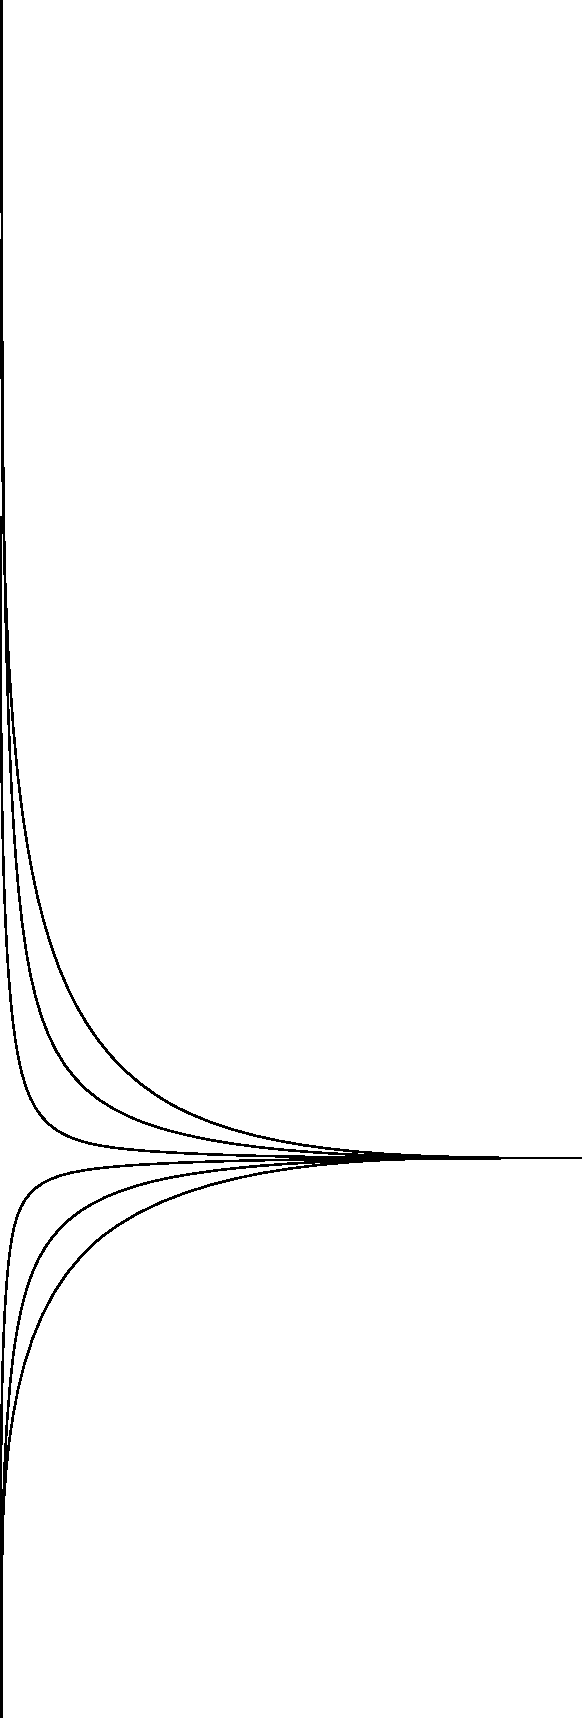
\includegraphics[scale=1.2]{pictures/title_drawing.pdf}
		%\end{figure}
		
	\end{center}
\end{titlepage}

%--- Inhaltsverzeichnis -------------------------------------
\newpage
% Inhaltsverzeichnis sichtbar machen
\setcounter{secnumdepth}{3} % Tiefe der Nummerierung
\setcounter{tocdepth}{3}    % Tiefe der Anzeige im Inhaltsverzeichnis
\setlength{\cftbeforetoctitleskip}{5pt} % Abstand vor dem Titel des Inhaltsverzeichnisses
\setlength{\cftaftertoctitleskip}{15pt} % Abstand nach dem Titel des Inhaltsverzeichnisses
\tableofcontents

%--- Abbildungsverzeichnis ----------------------------
\newpage
\setlength{\cftbeforeloftitleskip}{0pt} % Abstand vor dem Titel des Abbildungsverzeichnisses
\setlength{\cftafterloftitleskip}{15pt} % Abstand nach dem Titel des Abbildungsverzeichnisses
\listoffigures
\addcontentsline{toc}{section}{Abbildungsverzeichnis}  % Fügt es zum Inhaltsverzeichnis hinzu

% Hauptkapitel
%\setstretch{1.5}
\setstretch{1.6}
%\setstretch{2}
%--- Projektbeschreibung ------------------------------------
\newpage
\vspace{2mm}
\section{Einleitung}
\subsection{Abstract}
\subsection{Theorie}
\subsubsection{Das Prinzip des Linienstrahlers}
Ein jeder kennt die markanten Lautsprechersysteme von grösseren Eventveranstalltungen. Jedoch kennen nur die wenigsten deren Wirkungsweise, da immer mehr die visuellen Effekte im Vordergrund stehen. Jedoch könnte ein Stadion ohne diese Technologie wohl kaum effizient und in genügender Audioqualität beschallt werden.\\Die Wirkungsweise eines solchen \textit{Line Arrays} ist schnell erklärt: Mittel- und Hochtontreiber werden gleichmässig auf einer Linie angeordnet so dass sich durch Schallinterferenzen die einzelnen Wellensignale gezielt gegenseitig auslöschen und dadurch akustische Energie nur in bestimmte Richtungen abgestrahlt wird. \\Wie so oft ist dieser Effekt allerdings von mehreren Faktoren abhängig: Zum einen verschieben sich mit einer Änderung der Frequenz alle Phasenlagen, so dass sich alle Auslöschungszonen verschieben. Zum anderen spielen die genauen Dimensionen, Charakteristiken und Abstände zwischen den einzelnen Klangquelle eine entscheidende Rolle. So wirkt ein Line Array nur in einem bestimmen Frequenzband als Linienstrahler. Unterhalb dieses Frequenzbereichs interferieren die einzelnen Schallwellen wegen der langen Wellenlängen kaum noch und agieren mit tieferer Frequenz zunehmend als eine einzelne sphärische Schallquelle. Oberhalb des Frequenzbereiches ist die Wellenlänge kurz im Vergleich zu den Dimensionen der einzelnen Arrayelemente. Dadurch kommt es bereits zu Auslöschungen noch im Nahfeld des Elements, wodurch die Schallenergie direkt senkrecht abgestrahlt wird und nicht mehr mit dem restlichen Array interagiert.
{\color{red} ABBILDUNG SIMULATION}
\paragraph{Dynamisches Line Array}
Dieser  Durch geschickte Verzögerungen der elektrischen Signale lässt sich die Abstrahlcharakteristik auf modernen Linenstrahlern auch softwaremässig programmieren\footnote{\color{red}FOHNLINK}.
\paragraph{Dreidimensionales Beam Steering}
\subsubsection{Das Prinzip des Monochord}
\subsubsection{Signaltransport}
\subsubsection{Elektronische Klangerzeugung}

\subsection{Vorarbeiten}\label{vorarbeiten}
Vorgängig zu dieser Arbeit wurden einige Teile davon in Vorleistung angegangen. Dies mit dem Ziel, sich in der eigentlichen Projektzeit voll und ganz auf die Elektronik und ggf. die Software zu konzentrieren. Diese Vorarbeiten beinhalten darum hauptsächlich Konstruktions- sowie Testaufbauten und werden im folgenden aufgezeigt. Dementsprechend sind alle in Kapitel \ref{vorarbeiten} behandelten Komponenten und Tests als bereits vorhanden, bzw. als Ausgangslage anzusehen.
\subsubsection{Konstruktion und Herstellung Prototyp}
Um das mechanische Verhalten einer Saite und die Herstellungsmethode mit Lasergeschnittenem MDF zu testen, wurde ein Prototyp konstruiert und hergestellt. Dieser bestand aus einem Resonanzkasten mit einer einzelnen Saite, Steg sowie einer Halterung für einen Rundmagneten. Abbildung \ref{pics:prototype} zeigt ein 3D-Rendering der Konstruktion, welche in Autodesk Fusion 360 konstruiert wurde. Anschliessend wurden MDF-Platten mit einem CO2-Lasercutter des Fablab Winterthur zugeschnitten und diese dann aufeinander geleimt. Somit konnten schon erste Tests durchgeführt werden.
\begin{figure}[H]
	\centering
	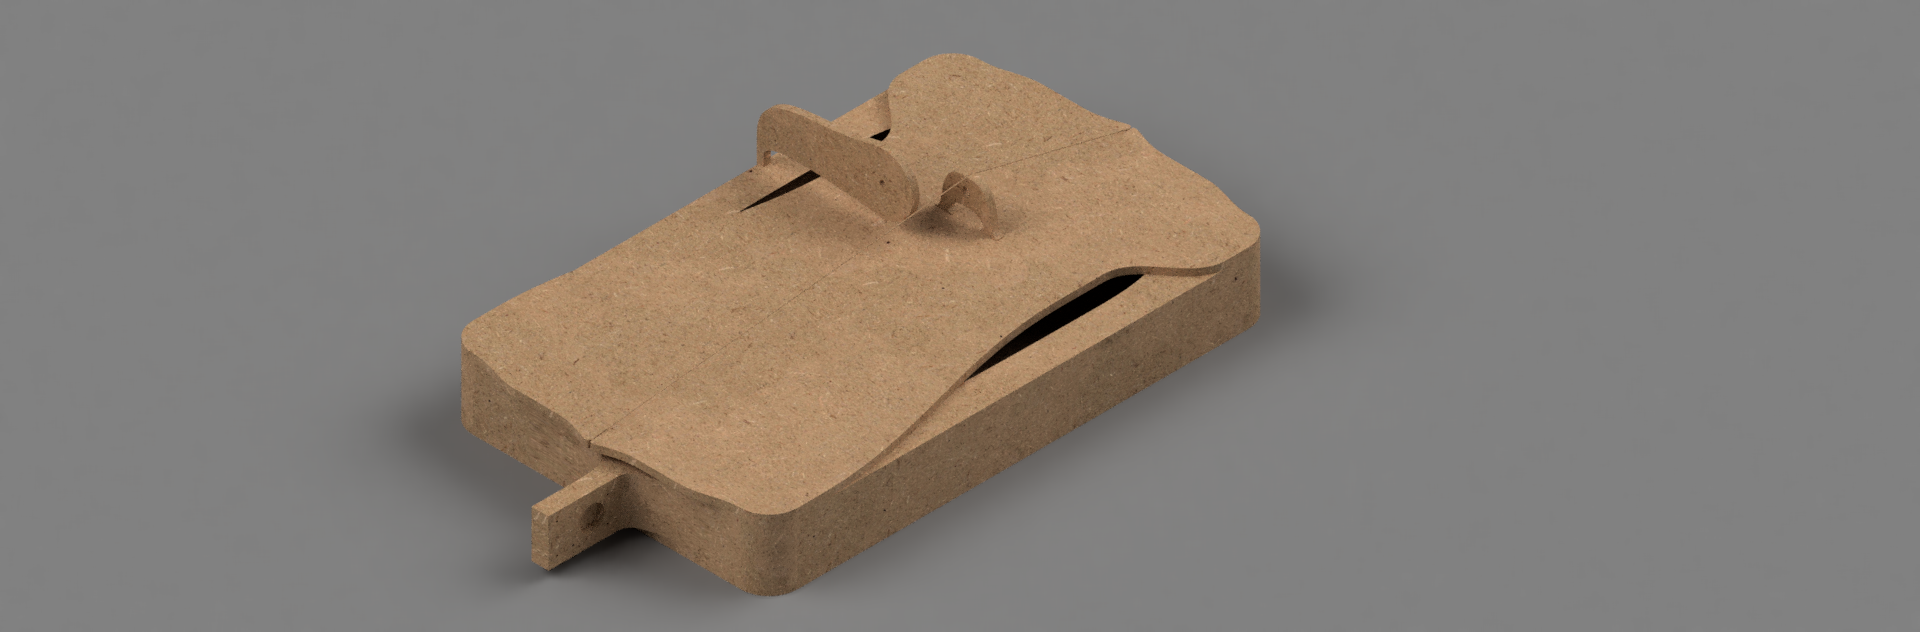
\includegraphics[width=\textwidth]{pictures/render_prototype.PNG}
	\caption{Rendering des Prototyps}
	\label{pics:prototype}
\end{figure}
\subsubsection{Schwingspulen}
Da noch unklar war, wie eine Saite am besten in Schwingung versetzt werden kann, wurden verschiedene Methoden getestet. Dabei wurden hauptsächlich drei Ansätze verfolgt:
\paragraph{Anregung mittels Schwingspule} Hierfür wurde Kupferdraht verschiedener Dicke um verschiedene Bobinen gewickelt und dann auf die Saite geleimt. Durch die Anwesenheit eines Magnetfeldes bewegt sich die Spule in Abhängigkeit des durchflossenen Stromes (Lorentzkaft). In Abbildung \ref{pics:all_voicecoils} sind einige Varianten aufgeführt. Getrieben wurde der Aufbau von einer analogen Endstufe. Hier zeigten sich schnell einige Herausforderungen: Oftmals war die Impedanz zu niedrig, oder die Hitzeentwicklung war zu stark. Ausserdem war ein grundsätzliches Problem, dass die Schwingspule sehr schnell zu rotieren begann, anstatt zu vibrieren und somit die Zuleitungen aufwickelte.
\begin{figure}[H]
	\centering
	\begin{subfigure}{0.7\textwidth}
		\centering
		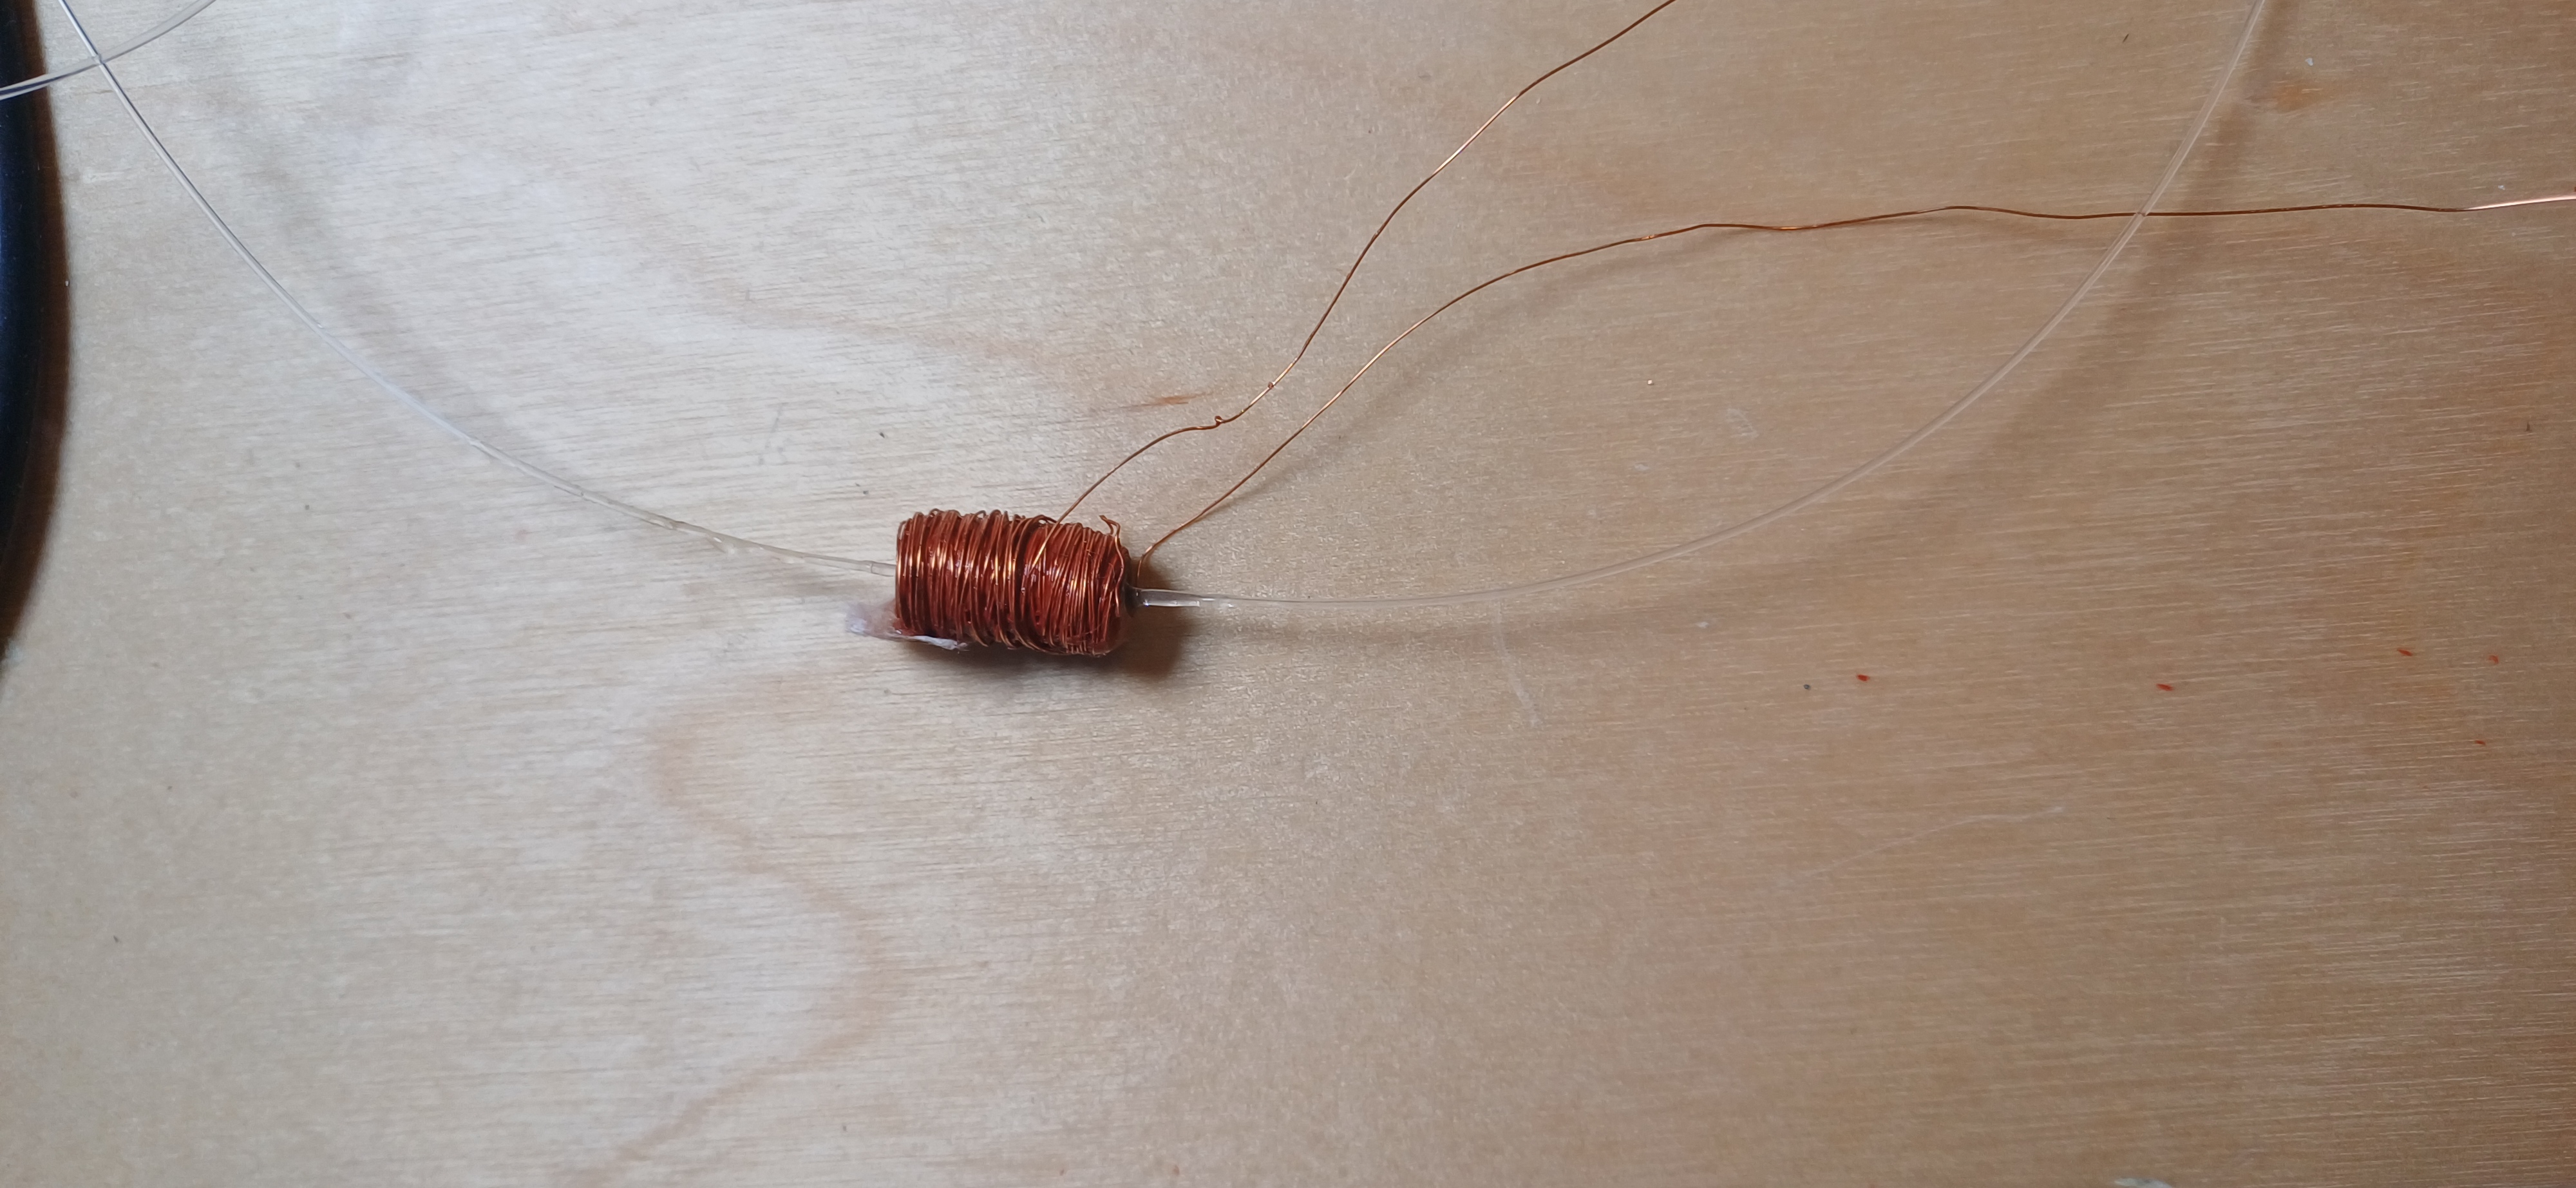
\includegraphics[width=\textwidth]{pictures/Schwingspule_lang.jpg}
		\caption{lange Schwingspule auf 5 Polymerbobinen}
		\label{pics:voicecoil_long}
		\vspace{4mm}
	\end{subfigure}\\
	\begin{subfigure}{0.7\textwidth}
		\centering
		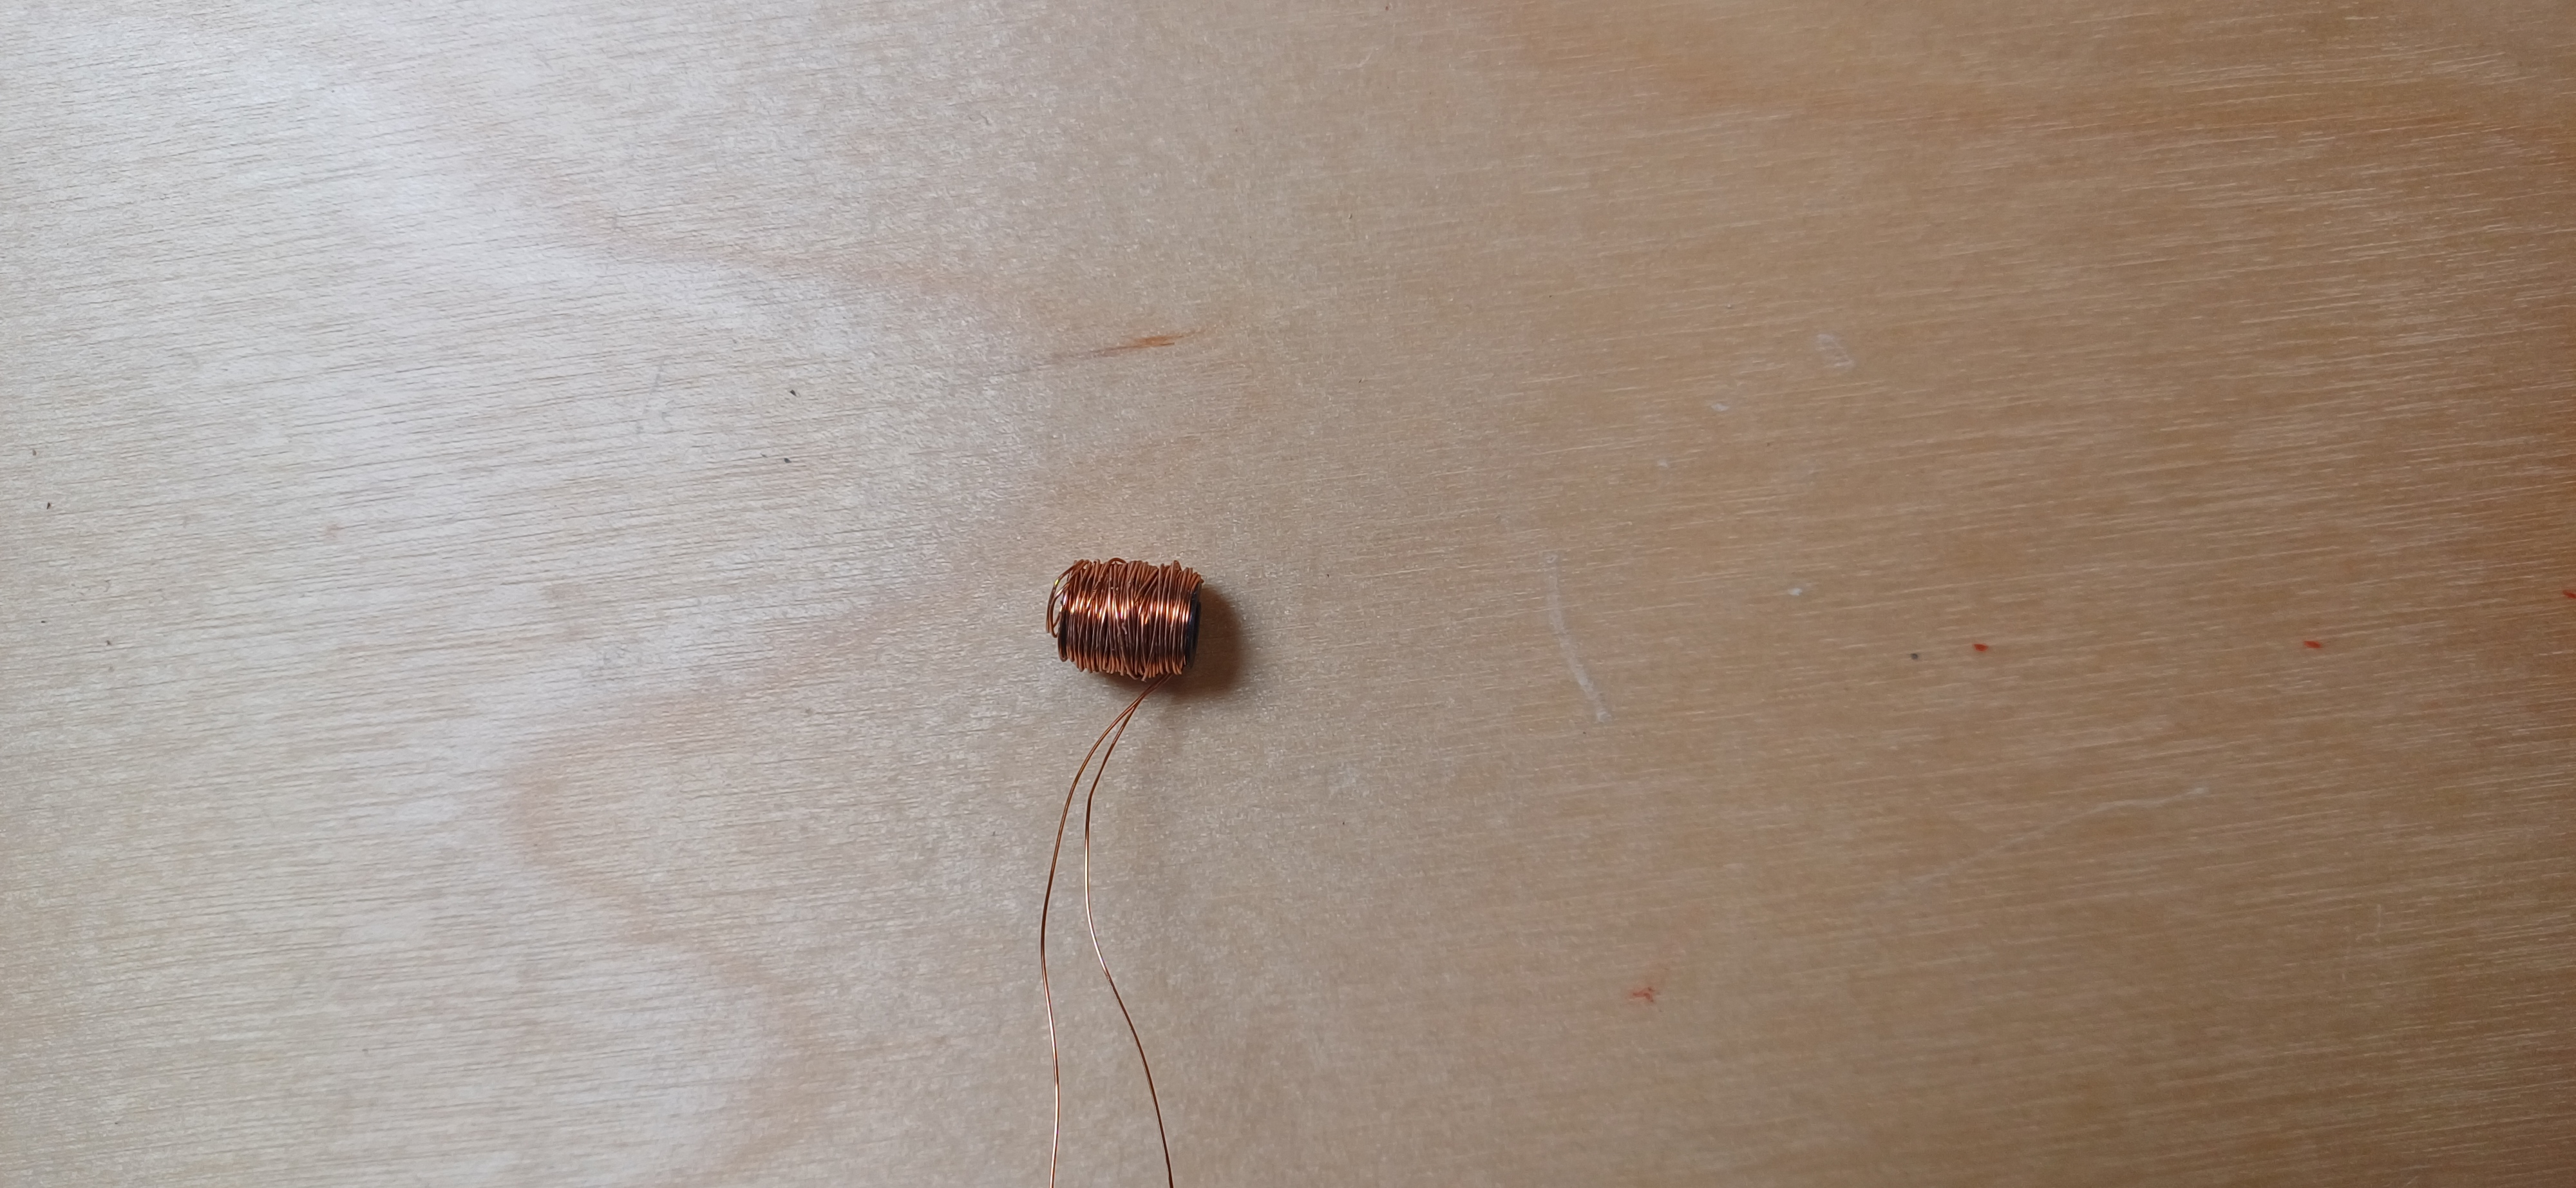
\includegraphics[width=\textwidth]{pictures/Schwingspule_kurz.jpg}
		\caption{kurze Schwingspule auf 3 Polymerbobinen}
		\label{pics:voicecoil_short}
		\vspace{4mm}
	\end{subfigure}\\
	\begin{subfigure}{0.7\textwidth}
		\centering
		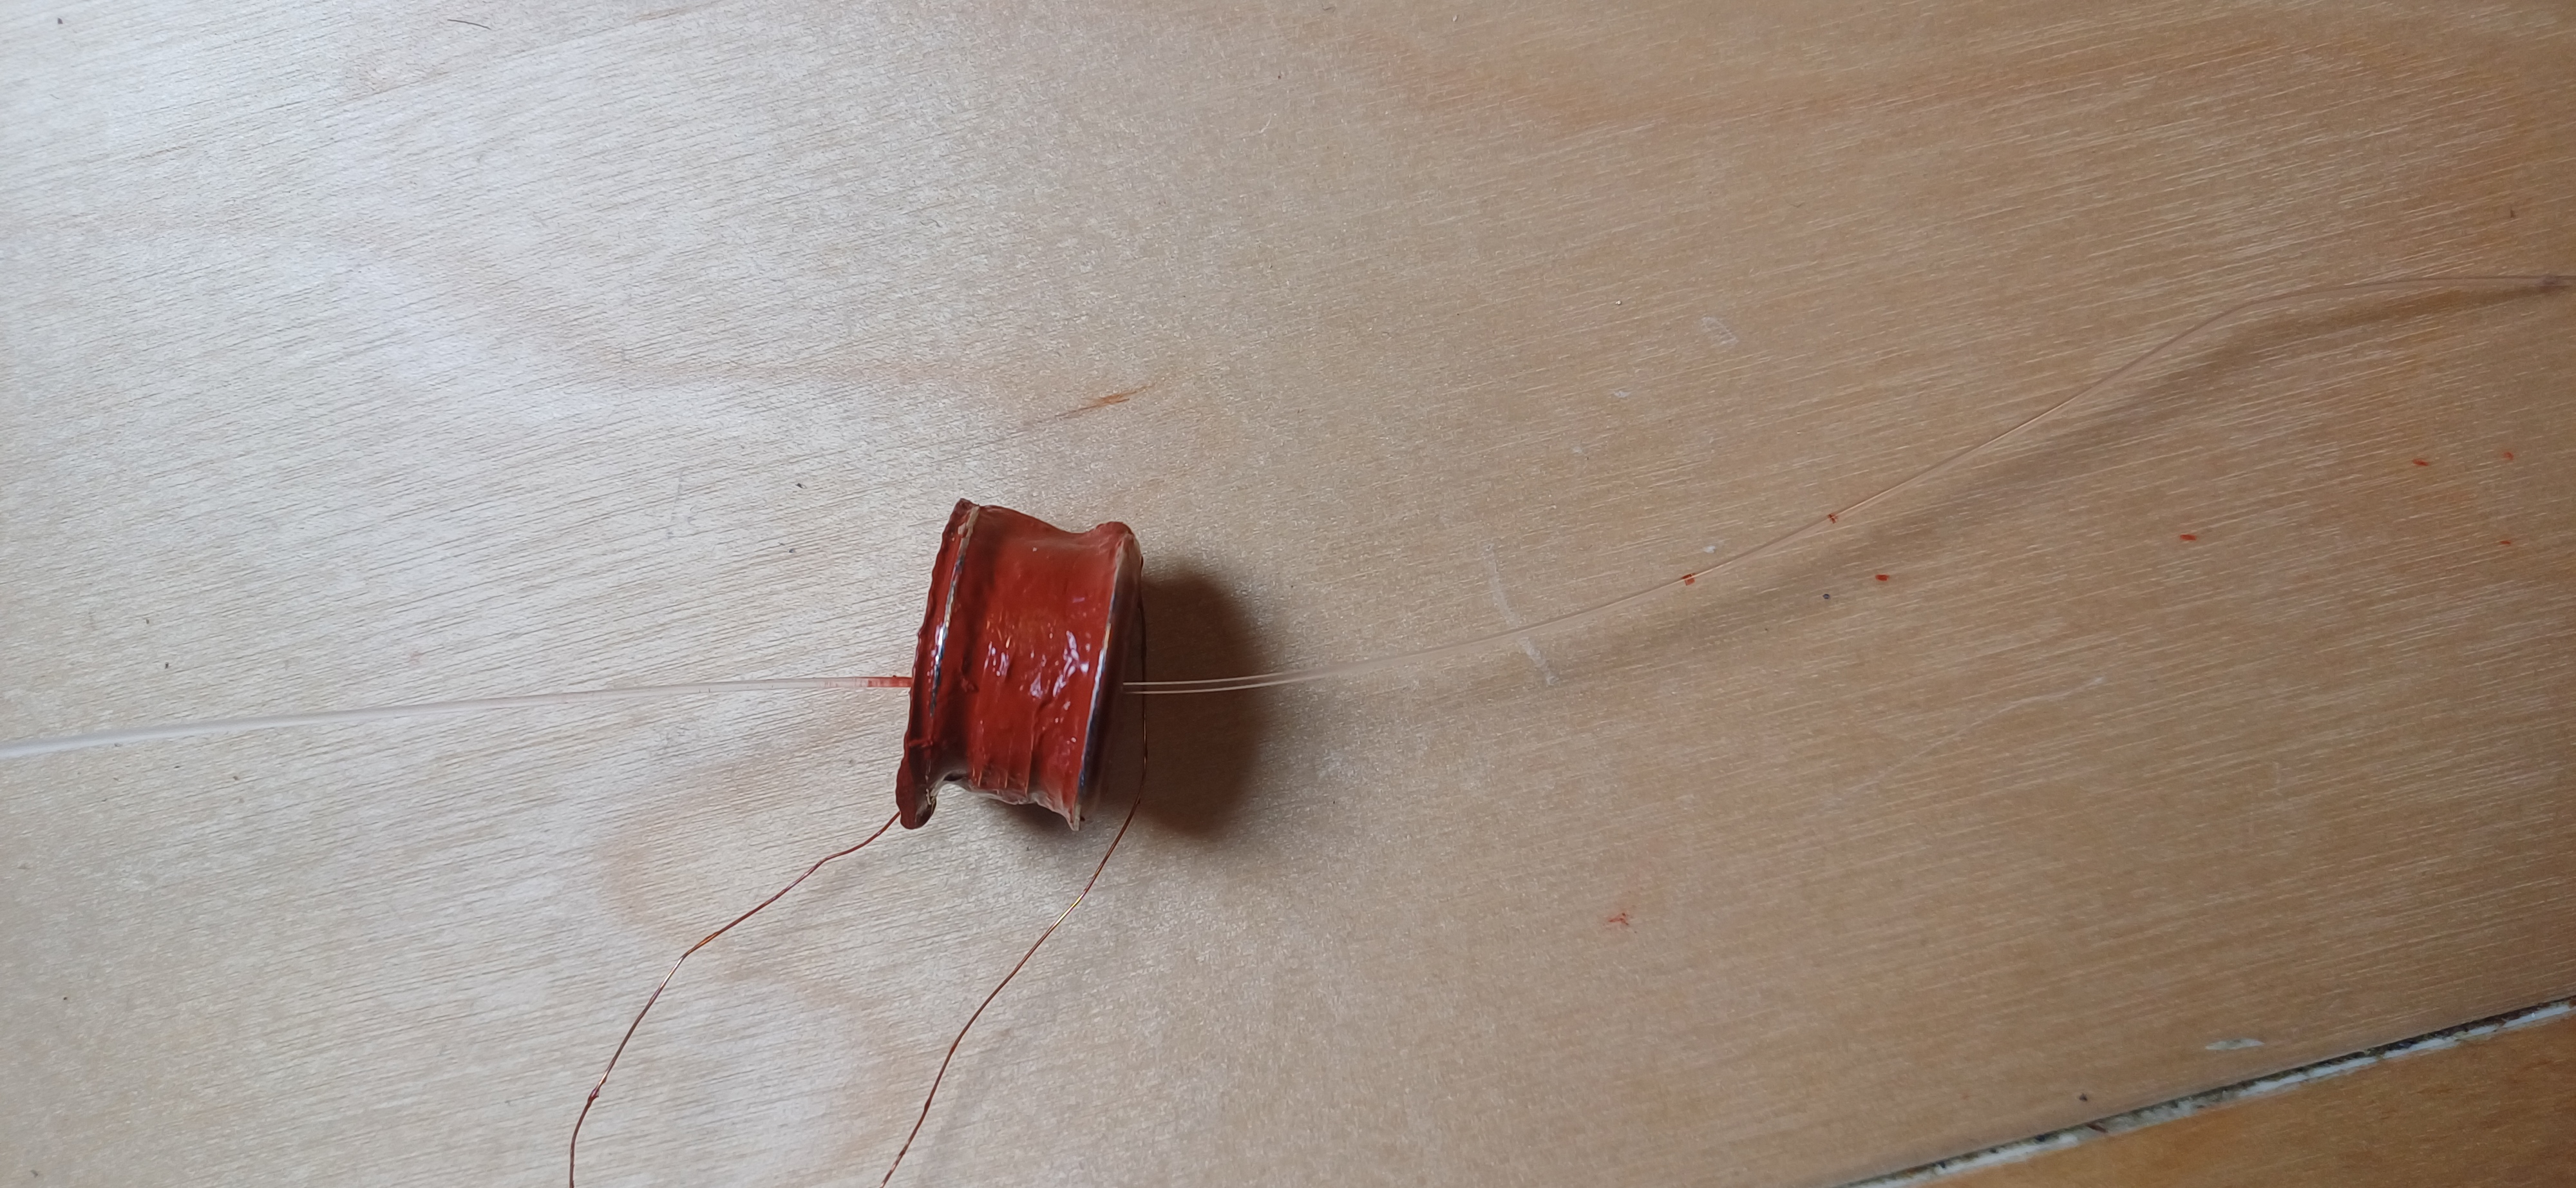
\includegraphics[width=\textwidth]{pictures/Schwingspule_eisenbobine.jpg}
		\caption{Schwingspule mit Eisenbobine, vergossen mit hitzebeständigem Kautschuk}
		\label{pics:voicecoil_iron}
		\vspace{4mm}
	\end{subfigure}
	\caption{verschiedene Schwingspulentypen}
	\label{pics:all_voicecoils}
\end{figure}
\noindent Des weiteren zeigte sich, dass ein einzelner Magnet neben einer Schwingspule die Spule nicht genügend mit einem Magnetfeld umschliesst. Die Bewegung blieb so sehr schwach. Weitaus besser funktionierte der Aufbau als zwei Magnete parallel montiert wurden und die Saite mit der Schwingspule dazwischen geführt wurde. So erzeugte die Schwingspule mit der Eisenbobine eine sehr starke Bewegung, konnte aber wegen des Rotationsproblems nicht verwendet werden.
\paragraph{Anregung mittels blanker Saite}
Eine sehr einfache Methode war es dann, den Signalstrom schlichtweg direkt durch die Saite zu leiten. Dabei wurde eine alte Instrumentensaite auf den Prototypen gespannt und Kontaktklemmen an den Enden angebracht. Zufälligerweise hatte die Saite eine Impedanz von ca. 3.2\Omega, wodurch sie direkt mit der Endstufe getrieben werden konnte.\\Dieser Aufbau hatte allerdings andere Limitationen: Ohne Wicklungen und Eisenkern blieb das erzeugte Magnetfeld der Saite sehr schwach. Zudem reagiert dieser Aufbau sehr stark auf die Resonanzfrequenz und deren harmonische Schwingungen, während andere Frequenzen kaum hörbar sind. {\color{red} VIDEO SWEEP} Somit liegt ein stark nicht-linearer Frequenzgang vor.
\begin{wrapfigure}{r}{0.5\textwidth}
	\vspace{10mm}
	\centering
	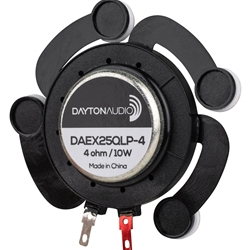
\includegraphics[scale=0.6]{pictures/exciter.jpg}
	\caption{DAEX25QLP-4 Exciter von Dayton Audio}
	\label{pics:exciter}
\end{wrapfigure}
\paragraph{Anregung mittels Exciter}
Ein weiterer Versuch bestand darin, einen Exciter, also sozusagen einen Lautsprecher ohne Membrane, auf den Prototypen zu platzieren. Somit wäre natürlich die Saite obsolet und der Begriff eines Saiteninstrument wohl nicht mehr zutreffend. Nichtsdestotrotz zeigte sich, dass dieser Aufbau um mehrere Zehnerpotenzen effektiver, also bisweilen auch ohrenbetäubend laut war. Auf der Innenseite montiert wäre das ganze Instrument schlichtweg eine unscheinbare Box welche auf Knopfdruck Klang abstrahlt\footnote{Das Prinzip existiert bereits als dekorative \textit{Flat Panel} oder \textit{Invisible Loudspeakers}}.
\subsubsection{Erkenntnisse}
\subsubsection{Konstruktion Korpus mit sechs Elementen}
\section{System Engineering}
\section{Situationsanalyse}
Als erster Schritt wurden einige Fakten und Rahmenbedingungen zum Projekt ausgelegt und so das Umsystem definiert.
\begin{itemize}
	\item Die Grundmotivation Projekts ist hauptsächlich ästhetischer Natur.
	\item Es bietet (voraussichtlich) weder marktwirtschaftlicher noch funktionellen Nutzen.
	\item Es besteht auch kein Auftraggeber- oder Kundenverhältnis in dem Sinne, und somit auch keine damit verknüpften Interessen.
	\item Markteinführung nicht zwingend, daher auch keine Zielgruppen bzw. Benutzer per se.
	\item Es liegt in dem Sinne auch kein systematisches Problem vor, welches gelöst werden soll.
	\item Das Projekt soll innerhalb von 14 Wochen realisiert werden.
	\item Es wurden bereits einige Vorarbeiten als Vorleistung getätigt (siehe \ref{vorarbeiten}).
	\item Zum Zeitpunkt der Arbeit sind aufwändige physikalische Simulationsprogramme wie COMSOL o.ä. nicht oder nur beschränkt verfügbar.
	\item Zudem war kein Zugang zu einer anechoischen Kammer verfügbar, worin z.B. die Abstrahlcharakteristik sehr genau hätte gemessen werden können.
	\item Als Produktionsstandort stand das FabLab Winterthur zur Verfügung.
	\item Die Firma \href{https://www.joyned.at/}{JOYNED GmbH} \begin{minipage}{3cm}
		\vspace{-1mm}
		
\includegraphics[scale=1.5]{pictures/joyned_logo.png}
	\end{minipage} erklärte sich bereit, ihr Fachwissen und Beratung zur Implementierung ihrer MILAN-Software zur Verfügung zu stellen.
\end{itemize}
\subsection{SWOT Analyse}
Anhand der gegebenen Aufgabenstellung wurde nun eine SWOT-Analyse durchgeführt, in der die Ausgangslage nach Stärken (\textit{strenghts}), Schwächen (\textit{weaknesses}), Chancen (\textit{opportunities}) und Gefahren (\textit{threats}) kategorisiert wurde. Diese sind in Abbildung \ref{pics:swot}  abgebildet und zeigten deutlich, das die Ausgangslage geprägt ist von Schwächen, jedoch für die Zukunft überwiegen Chancen bereitstellt. Die der Ist-Zustand konnte somit als \textit{High Risk - High Reward} Situation bezeichnet werden.
\begin{figure}[H]
	\centering
	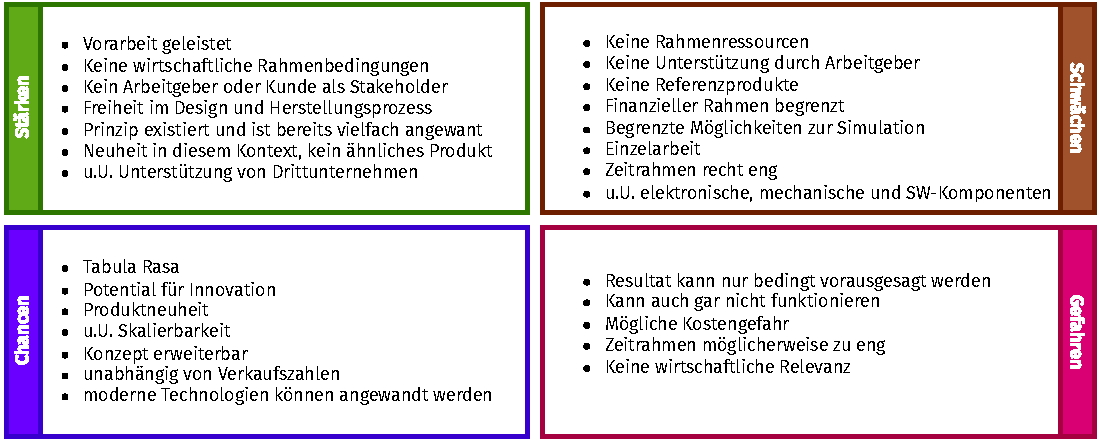
\includegraphics[width=\textwidth]{pictures/SWOT.pdf}
	\caption{SWOT-Analyse}
	\label{pics:swot}
\end{figure}
\subsection{Ishikawa Diagramm}
Die möglichen Problemursachen für das Projekt wurden nun kategorisiert und danach in Abbildung \ref{pics:ishikawa} aufgezeichnet. Es zeigte sich, dass sich die (möglichen) Problemursachen in folgende Oberkategorien aufteilen liessen:
\paragraph{Physik} Hier ist zum einen das grundlegende Phänomen, welches genutzt werden soll recht komplex und von vielen Faktoren abhängig. Zum anderen muss eine Saite in Schwingung versetzt werden, was physikalisch gesehen nicht unbedingt eine Effiziente Methode zur Klangerzeugung ist.
\paragraph{Material} Nebst den Faktoren wie Materialdichte, Gewicht und Nachgiebigkeit\footnote{siehe: \href{https://de.wikipedia.org/wiki/Compliance_(Physiologie)}{Compliance (Physiologie)}}, spielte vor allem auch die Herstellungsmöglichkeiten eine Rolle: Wie kann ein Material in welchen Dimensionen produziert werden?
\paragraph{Engineering} Hier ist vor allem die Hardware- und Software zu nennen. Je nach Variante können dabei keines, eines oder beide obsolet werden. Zudem können aus der Signalübertragung her auch Fehlerquellen entstehen.
\paragraph{Zeit} Der Zeitfaktor gilt wohl als grösster Problemverursacher, da der Abgabetermin fix vorgegeben ist und nicht verschoben werden kann.
\paragraph{Budget} Da kein Auftraggeber oder Firma als finanzielle Unterstützung vorhanden ist, muss das ganze Projekt aus privaten Reserven finanziert werden.
\paragraph{Produktesicherheit} Obwohl das Produkt nicht direkt als Verkaufsprodukt vorgesehen ist, muss die Sicherheit doch als Faktor miteinbezogen werden.
\vspace{6mm}
\begin{figure}[H]
	\centering
	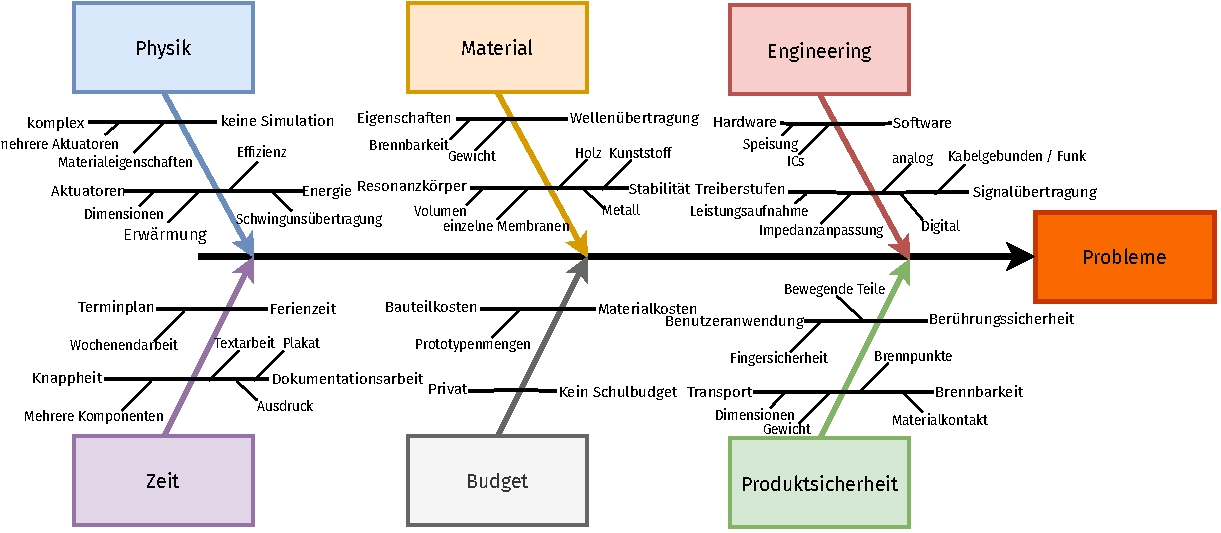
\includegraphics[width=\textwidth]{pictures/ishikawa.pdf}
	\caption{Ishikawa-Analyse}
	\label{pics:ishikawa}
\end{figure}
\section{Zieldefinition}
Das Grundlegende Projektziel ist eigentlich sehr einfach beschrieben: Es soll ein Gerät entwickelt werden, welches den Klang in eine bestimmte Richtung abstrahlen kann (Beam Forming). Da jedoch in Rahmen dieser Ausbildung bzw. dieses Projekts keine anechoische Kammer und/oder eine genau winkelverstellbare Halterung zur Verfügung stand, um die Direktionalität des Schallpegels zu messen, war die grundsätzliche Messbarkeit dieses Zieles fraglich.\\Nichtsdestotrotz sollen sowohl das oben genannte Hauptziel (\textbf{Muss}) als auch Nebenziele (\textbf{Soll, Kann}) an dieser Stelle definiert und quantifiziert werden. Dabei ist der Ziel-Zeitpunkt jeweils der Abgabetermin der Arbeit. Tabelle \ref{tab:aims} zeigt die verschiedenen Ziele und deren Messgrössen.\\
\begin{table}[H]
	\centering
	%\rowcolors{2}{gray!0}{gray!8}
	\setstretch{1.5}
	\begin{tabularx}{\textwidth}{l>{\columncolor{red!22}}c>{\columncolor{orange!12}}c>{\columncolor{blue!12}}cccc}
		\centering
		Zielbezeichnung & \textbf{MUSS} & \textbf{SOLL} & \textbf{KANN} & Messgrösse & Kenn/Grenzzahl & Bedingung  \\
		\hline
		{\Large \textbf A}\hspace{3mm}\begin{minipage}{2.4cm}
			\vspace{2mm}
			\setstretch{1.1}
			Direktionale Abstrahlung
			\vspace{2mm}
		\end{minipage} & x &  &  & Direktivität & -3dB SPL & \begin{minipage}{2.1cm}
			\vspace{1mm}
			\setstretch{1.1}
			\centering
			> 10° von Bezugsachse
		\end{minipage}\\
		\hline
		{\Large \textbf B}\hspace{3mm}\begin{minipage}{2.4cm}
			\vspace{2mm}
			\setstretch{1.1}
			Möglichst wenige Stecker
			\vspace{2mm}
		\end{minipage} &  & x &  & Anzahl Stecker & max. 3 & - \\
		\hline
		{\Large \textbf C}\hspace{3mm}\begin{minipage}{2.4cm}
			\vspace{2mm}
			\setstretch{1.1}
			Untere Grenzfrequenz tief genug
			\vspace{2mm}
		\end{minipage} &  & x &  & -3dB Punkt & min. 100 Hz & - \\
		\hline
		{\Large \textbf D.1}\hspace{1.5mm}\begin{minipage}{2.4cm}
			\vspace{2mm}
			\setstretch{1.1}
			Mobilität
			\vspace{2mm}
		\end{minipage} &  & x &  & Gewicht & max. 6 kg & - \\
		%\hline
		{\Large \textbf D.2}\hspace{1mm}\begin{minipage}{2.4cm}
			\vspace{2mm}
			\setstretch{1.1}
			Mobilität
			\vspace{2mm}
		\end{minipage} &  &  & x & Dimensionen & max. 1.8x0.8x0.3m & - \\
		\hline
		{\Large \textbf E}\hspace{3mm}\begin{minipage}{2.4cm}
			\vspace{2mm}
			\setstretch{1.1}
			Speisung + Daten auf einem Stecker
			\vspace{2mm}
		\end{minipage} &  &  & x & Anzahl Stecker & 1 & - \\
		\hline
		{\Large \textbf F}\hspace{3mm}\begin{minipage}{2.4cm}
			\vspace{2mm}
			\setstretch{1.1}
			Abstrahlung softwaremässig steuerbar
			\vspace{2mm}
		\end{minipage} &  &  & x & Möglich & Ja & -\\
		\hline
		{\Large \textbf G}\hspace{3mm}\begin{minipage}{2.4cm}
		\vspace{2mm}
		\setstretch{1.1}
		Reduziertes Brandrisiko
		\vspace{2mm}
		\end{minipage} & x &  &  & \begin{minipage}{2cm}
			\centering
			\vspace{2mm}
			MTBF (durch Brand)\vspace{2mm}
		\end{minipage} & min. 200 Jahre & \begin{minipage}{2.4cm}
		\vspace{1mm}
		\setstretch{1.1}
		\centering
		Sachgemässe Benützung
		\end{minipage}\\
		\hline
		{\Large \textbf H}\hspace{3mm}\begin{minipage}{2.4cm}
		\vspace{2mm}
		\setstretch{1.1}
		Benutzersicherheit
		\vspace{2mm}
		\end{minipage} &  & x &  & \begin{minipage}{2cm}
		\centering
		\vspace{2mm}
		MTBF (durch Benutzerunfall)
		\vspace{2mm}
		\end{minipage} & min. 80 Jahre & \begin{minipage}{2.4cm}
		\vspace{1mm}
		\setstretch{1.1}
		\centering
		Sachgemässe Benützung
		\end{minipage} \\
		\hline
		{\Large \textbf I}\hspace{3mm}\begin{minipage}{2.4cm}
		\vspace{2mm}
		\setstretch{1.1}
		Batteriebetrieben
		\vspace{2mm}
		\end{minipage} &  &  & x & Akkulaufzeit & 12h & - \\
		\hline
		{\Large \textbf J}\hspace{3mm}\begin{minipage}{2.4cm}
		\vspace{2mm}
		\setstretch{1.1}
		Drahtlose Signalübertragung
		\vspace{2mm}
		\end{minipage} &  &  & x & Funkstrecke & Ja & -
	\end{tabularx}
	\label{tab:aims}
	\caption{Projektziele}
\end{table}
\subsection{Zielbeziehungen}
Aus den beschriebenen Zielen können einige Widersprüche festgestellt werden:
\paragraph{C vs. D.2} Eine tiefe untere (akustische) Grenzfrequenz bedingt immer ein grösseres Volumen des Resonanzkörpers. Eine Mobilität bedingt eine gewisse \textit{Handlichkeit} bzw. Transportfähigkeit. Somit setzten sich diese Ziele direkt im Widerspruch.
\paragraph{I vs. G} Je nach Batterietyp können diese sehr wohl ein Risiko der Brennbarkeit bergen. Somit ist mit einer Batterie automatisch die Brennbarkeit erhöht.
Allerdings ergab sich auch ein sich ergänzendes Zielpaar:
\paragraph{B vs. E} Beide Ziele haben im Endeffekt den selben Fokus. Eine ideale Erfüllung wäre hier ein einziger Stecker mit Speisung und Datensignalen.
\section{Zielgewichtung}\label{sec:zielgewichtung}
Anschliessend wurden die Ziele jeweils gegeneinander verglichen und eines davon als Präferenz ausgewählt. Somit entstand eine in Tabelle \ref{tab:aimweights} ersichtliche Präferenzmatrix. Aus den Anzahl gewonnenen Vergleichen kann nun pro Ziel ein Rang und eine Gewichtung ermittelt werden.
\begin{table}[!ht]
	\centering
	%\rowcolors{2}{gray!0}{gray!8}
	\begin{tabularx}{\textwidth}{cccclccccc}
		\toprule
		\textbf{Rang} & \textbf{Gewicht} & \textbf{Anzahl} & \multicolumn{2}{c}{\textbf{Zielbezeichnung}} & \multicolumn{4}{c}{\textbf{Präferenzen}} \\ \midrule
		\textbf{2} & 18 & 4 & \textbf{A} & Direktionale Abstrahlung & ~ & ~ & ~ & ~ & ~ \\ 
		\textbf{} & ~ & ~ & ~ & ~ & A & ~ & ~ & ~ & ~ \\ 
		7 & 5 & 1 & \textbf{B} & Möglichst wenige Stecker & ~ & A & ~ & ~ & ~ \\ 
		\textbf{} & ~ & ~ & ~ & ~ & B & ~ & A & ~ & ~ \\ 
		9 & 0 & 0 & \textbf{C} & Untere Grenzfrequenz tief genug & ~ & D.1 & ~ & ~ & ~ \\ 
		\textbf{} & ~ & ~ & ~ & ~ & D.1 & ~ & ~ & ~ & ~ \\ 
		4 & 9 & 2 & \textbf{D.1} & Mobilität (Gewicht) & ~ & ~ & ~ & A & ~ \\ 
		\textbf{} & ~ & ~ & ~ & ~ & D.2 & ~ & ~ & ~ & ~ \\ 
		\textbf{2} & 18 & 4 & \textbf{D.2} & Mobilität (Dimensionen) & ~ & D.2 & ~ & ~ & ~ \\ 
		\textbf{} & ~ & ~ & ~ & ~ & D.2 & ~ & D.2 & ~ & G \\ 
		9 & 0 & 0 & \textbf{E} & Speisung+Daten auf einem Stecker & ~ & F & ~ & ~ & ~ \\ 
		\textbf{} & ~ & ~ & ~ & ~ & F & ~ & ~ & ~ & ~ \\ 
		4 & 9 & 2 & \textbf{F} & Abstrahlung softwaremässig steuerbar & ~ & ~ & ~ & G & ~ \\ 
		\textbf{} & ~ & ~ & ~ & ~ & G & ~ & ~ & ~ & ~ \\ 
		\textbf{1} & 27 & 6 & \textbf{G} & Reduziertes Brandrisiko & ~ & G & ~ & ~ & ~ \\ 
		\textbf{} & ~ & ~ & ~ & ~ & G & ~ & G & ~ & ~ \\ 
		4 & 9 & 2 & \textbf{H} & Benutzersicherheit & ~ & ~ & ~ & ~ & ~ \\ 
		\textbf{} & ~ & ~ & ~ & ~ & H & ~ & ~ & ~ & ~ \\ 
		9 & 0 & 0 & \textbf{I} &  Batteriebetrieben & ~ & H & ~ & ~ & ~ \\ 
		\textbf{} & ~ & ~ & ~ & ~ & J & ~ & ~ & ~ & ~ \\ 
		7 & 5 & 1 & \textbf{J} &  Drahtlose Signalübertragung & ~ & ~ & ~ & ~ & ~ \\ 
		\bottomrule
	\end{tabularx}
	\caption{Zielgewichtung}
	\label{tab:zielgewichtung}
\end{table}
Somit konnten die drei Hauptziele eruiert werden:
\paragraph{G Reduziertes Brandrisiko} Das Endprodukt muss ein möglichst minimiertes Brennbarkeitsrisiko aufweisen. Zwar gibt es mit der EN 13501-1 eine Klassifikation zum Brandverhalten, jedoch behandelt dieses rein Baustoffe und nicht ein Produkt als ganzes. Dieses Ziel ist insbesondere relevant, da u.U. Brennbare Materialen wie MDF in Kombination von Leistungsendstufen vorkommen.
\paragraph{D.2 Mobilität}
\paragraph{A Direktionale Abstrahlung}
\section{Variantendefinition}
\subsection{Morphologischer Kasten}
Da das Projekt mehrere Ebenen(Elektronisch, mechanisch und Signaltechnisch) umfasst, wurde versucht, alle Möglichkeiten zu jedem Sub-Element in einem morphologischen Kasten aufzuzeichnen. Dieser ist in Abbildung \ref{pic:morphologischer_kasten} zu sehen. Aus diesen konnten nun verschiedene Varianten generiert und bewertet werden.
\begin{figure}[H]
	\includegraphics[width=\textwidth]{pictures/morphologischer_kasten.pdf}
	\caption{Der morphologische Kasten}
	\label{pic:morphologischer_kasten}
\end{figure}
\subsubsection{Variante A: Alles Analog}
In dieser Variante wird möglichst alles via analoge Signalpfade geführt. So kann zum Beispiel die Signalverzögerung durch Allpass-Filter realisiert werden. Fokus ist auf Robustheit und Signalreinheit.
\begin{figure}[H]
	\centering
	\includegraphics{pictures/VarianteA_allesAnalog.pdf}
	\caption{Variante A}
\end{figure}
\paragraph{Vorteile} Resultate sind relativ schnell messbar. Programmierarbeit erübrigt sich komplett. Zudem sind rein analoge Designs tendenziell robuster und langlebiger. Durch die fehlende Abtastung bleiben Höhenanteile erhalten und die Signalqualität eher hochwertiger.
\paragraph{Nachteile} Fehlersuche ist rein messtechnisch möglich. Nachträgliche Änderungen sehr teuer und Zeitaufwändig. Der Überwachung sind starke Grenzen gesetzt: So muss bei einem Unterbruch der gesamte Signalpfad durchgemessen werden. Ein weiterer Nachteil ist die Schwingspule, deren Befestigung an der Saite noch genauer ausgearbeitet werden muss.
\newpage
\paragraph{Risikoanalyse}
Durch sich bewegende Teile, welche unter Umständen durch den Benutzer berührt werden können entsteht zum einen ein Risiko einer leichten Verletzung. Zum anderen könnte die physikalische Montage von analoger Leistungselektronik auf MDF zu einer Brandgefahr führen. Zudem können sehr leicht durch fehlende, unsaubere oder falsche Steckverbindungen Funktionsfehler auftreten. Mit der noch offenen Montagetechnik der Schwingspule besteht zudem die Gefahr, dass die Klangerzeugung nicht überzeugend funktioniert, insbesondere im Dauereinsatz.
\begin{figure}[H]
	\centering
	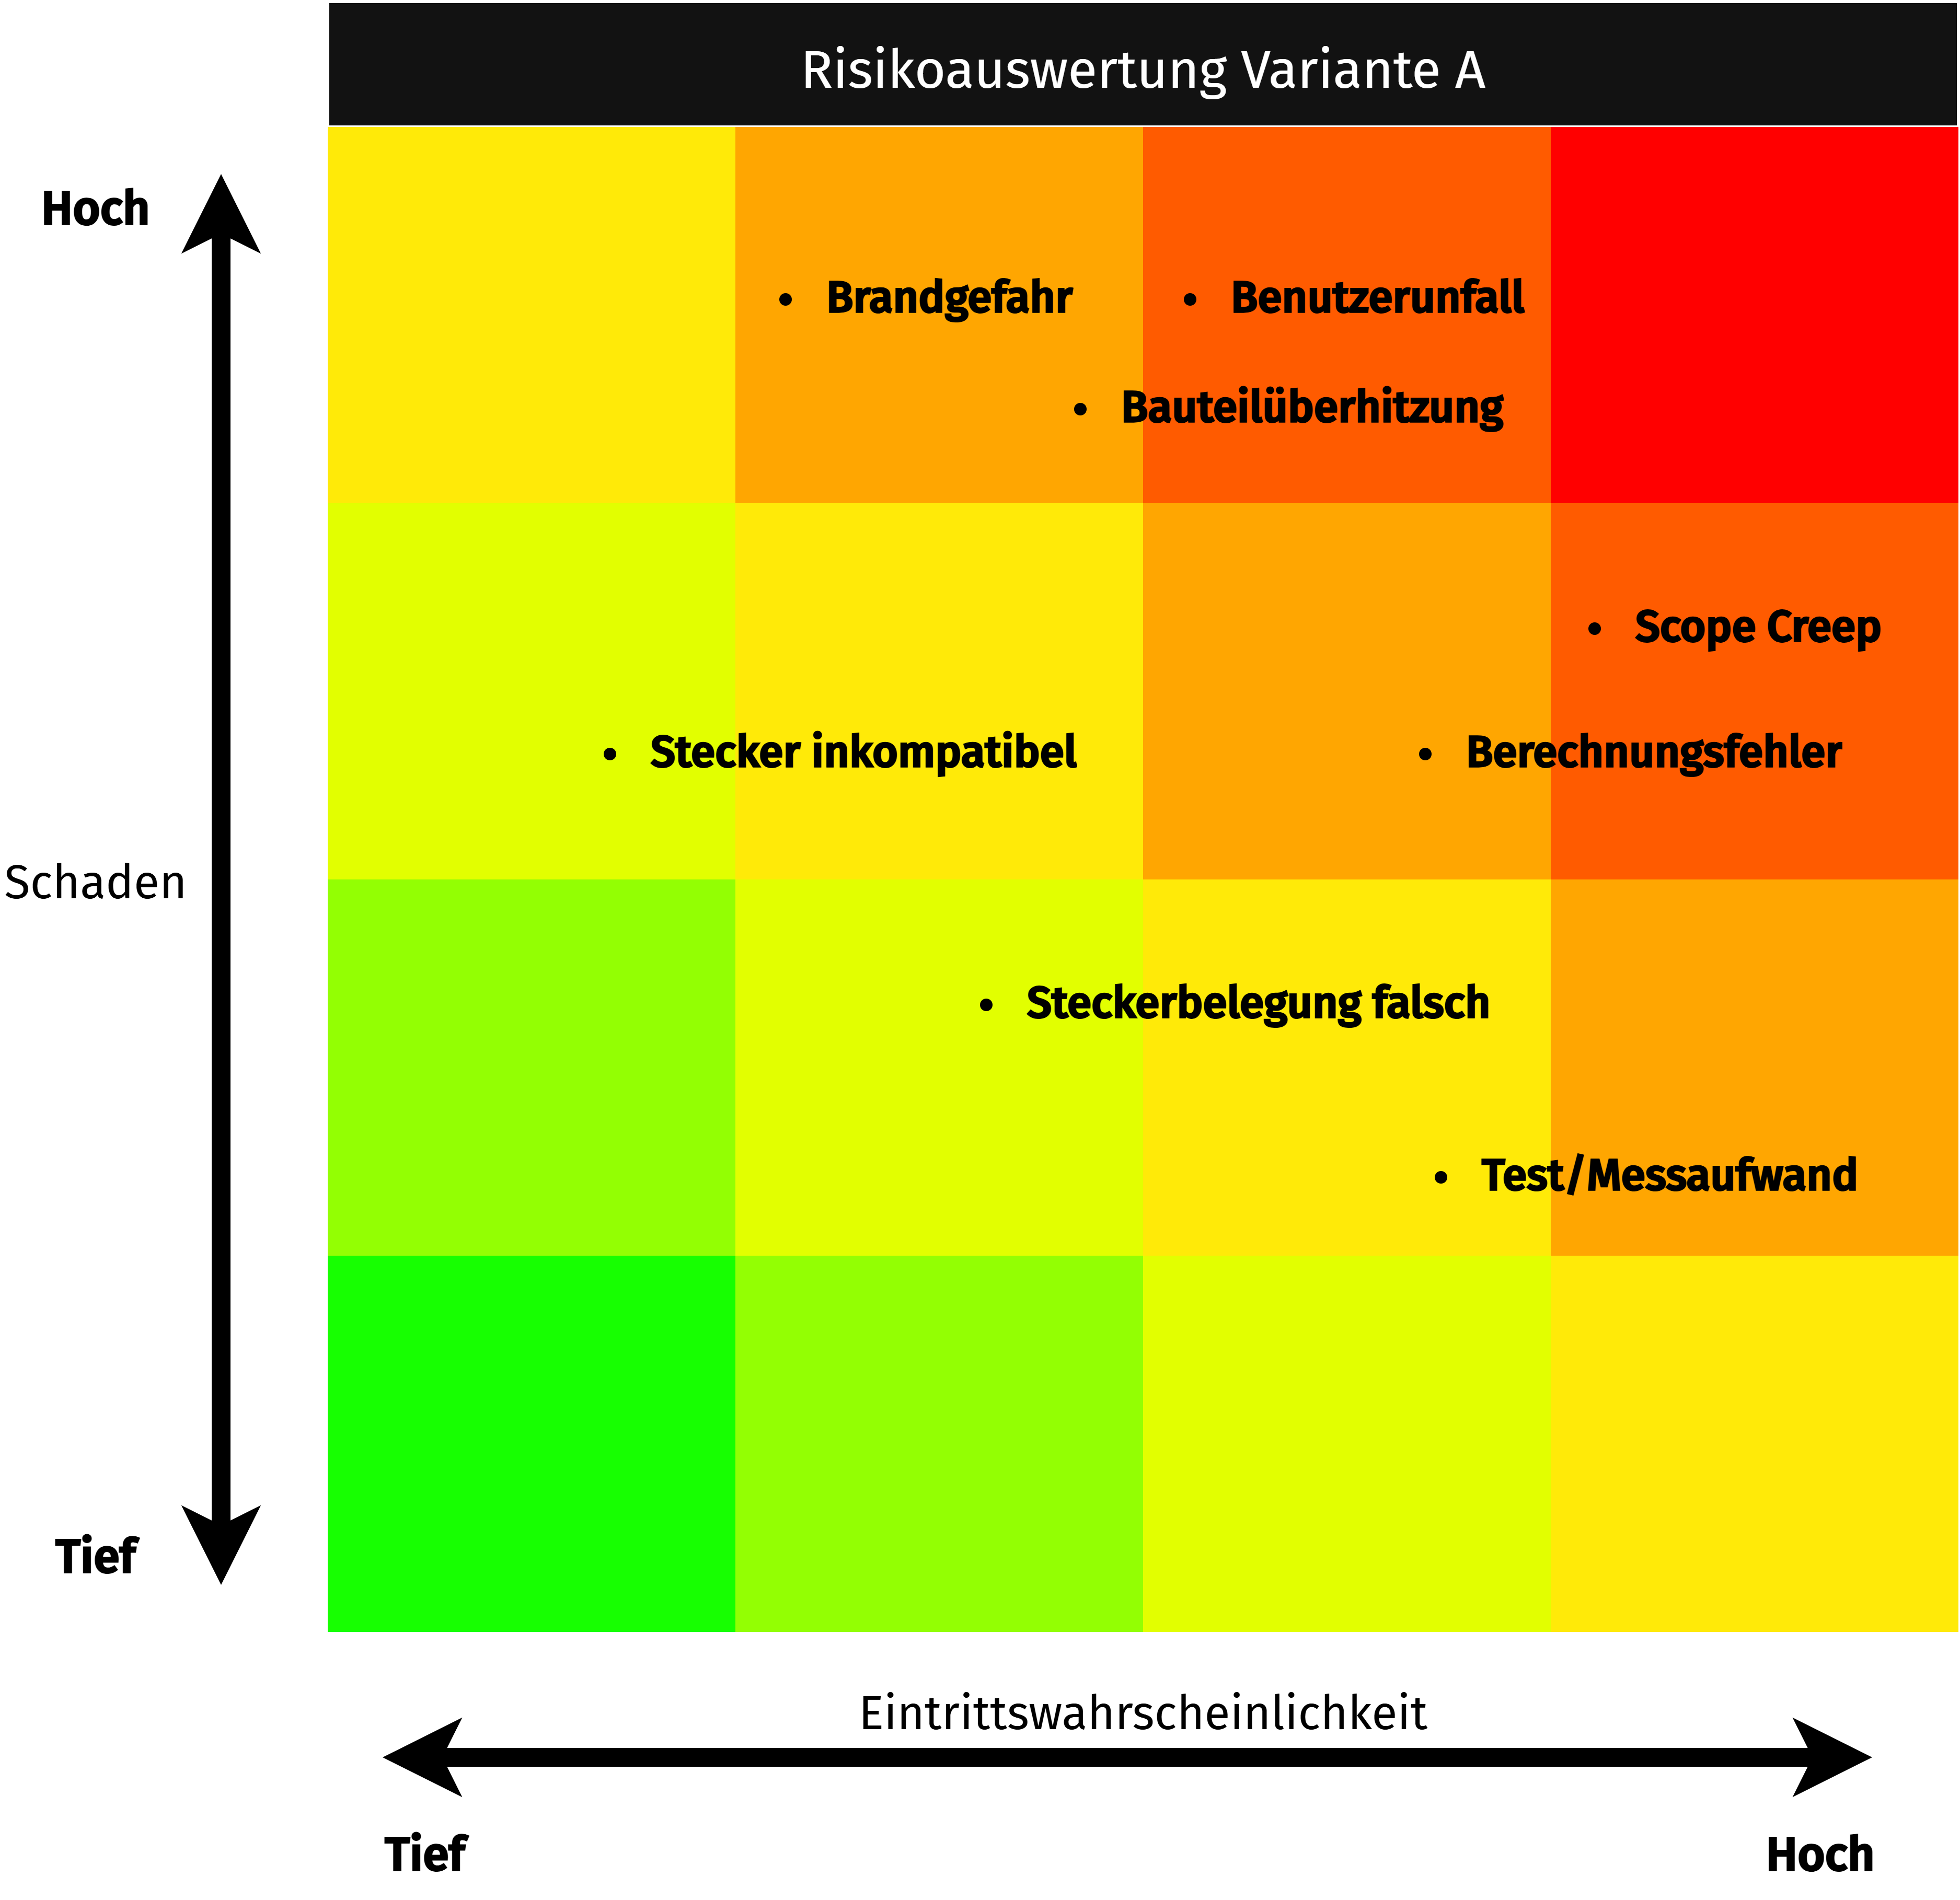
\includegraphics[width=\textwidth*4/5]{pictures/risks-Variante A_ Alles analog.png}
	\caption{Risikoanalyse der Variante A}
\end{figure}
\newpage
\subsubsection{Variante B: Drahtlos \& Portabel}
Der Hauptfokus dieser Variante ist maximale mobilität und minimale Steckverbindungen. Dies wird zum einen durch ein Batterie erreicht, und zum anderen durch eine drahtlose Signalübertragung.
\begin{figure}[H]
	\centering
	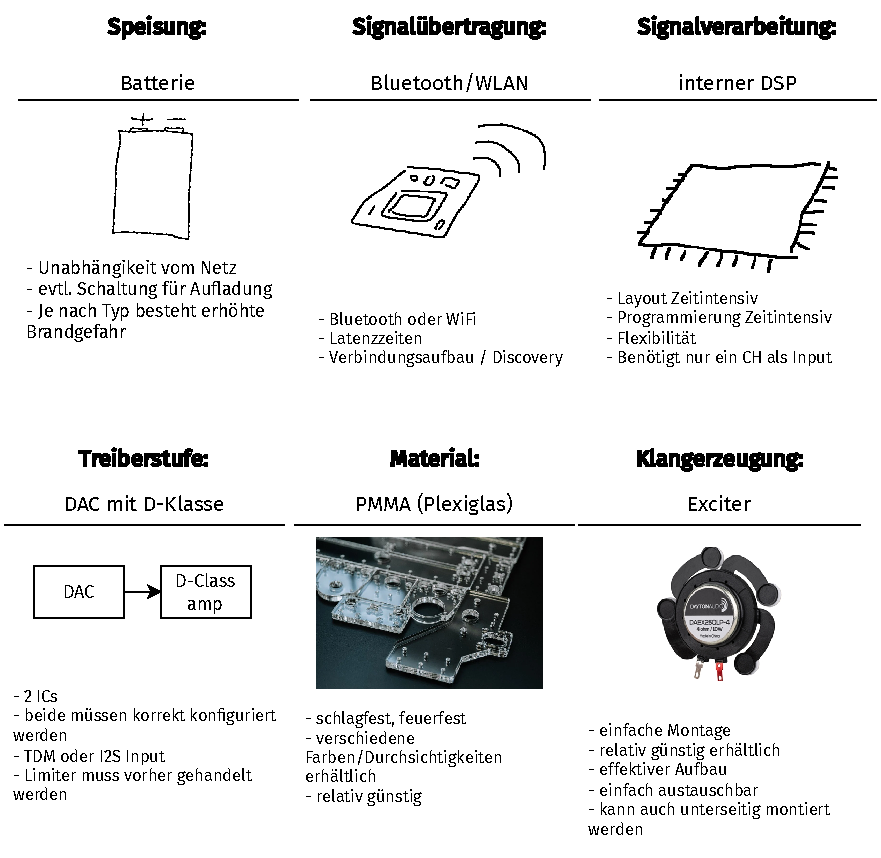
\includegraphics{pictures/VarianteB_drahtlosPortabel.pdf}
	\caption{Variante B}
\end{figure}
\paragraph{Vorteile} Da hier die Datenübertragung ohne Stecker auskommt, kann hier im Einsatz komplett auf Kabel verzichtet werden. Somit vereinfachen sich insbesondere weiträumigere Setups, in dem das Gerät weiter weg aufgestellt ist. Als einziger Stecker bleibt ein Ladestecker für die Batterie übrig. Für die Einbindung von Batterien bzw. deren Ladezyklus gibt es zudem bereits sehr viele fertige Komponenten.
\paragraph{Nachteile} Die korrekte Implementierung des Signalpfades von Bluetooth oder Wifi über DSP, den DAC und die D-Klasse Endstufe wird wohl einiges an Aufwand brauchen, insbesondere bei zeitkritischen Anwendungen wie dieser. Zudem entsteht je nach Batterietyp eine Brandgefahr, die zwar durch das Plexiglas vermindert ist aber dennoch z.B. andere Materialien im Raum in Brand setzen kann.
\newpage
\paragraph{Risikoanalyse}
Zwar entfällt hier das Risiko einer falschen Steckverbindung komplett, jedoch erhöht sich durch die Anwesenheit einer Batterie die Brandgefahr deutlich. Dies auch wenn PMMA als Material verwendet wird, da sich die Batterie selbst schon entzünden kann. Zudem entsteht durch den komplexen Aufbau ein unter Umständen zeitintensive Designphase, welche auch mit HF-Layoutfehlern verbunden sein können.
\begin{figure}[h]
	\vspace{1cm}
	\centering
	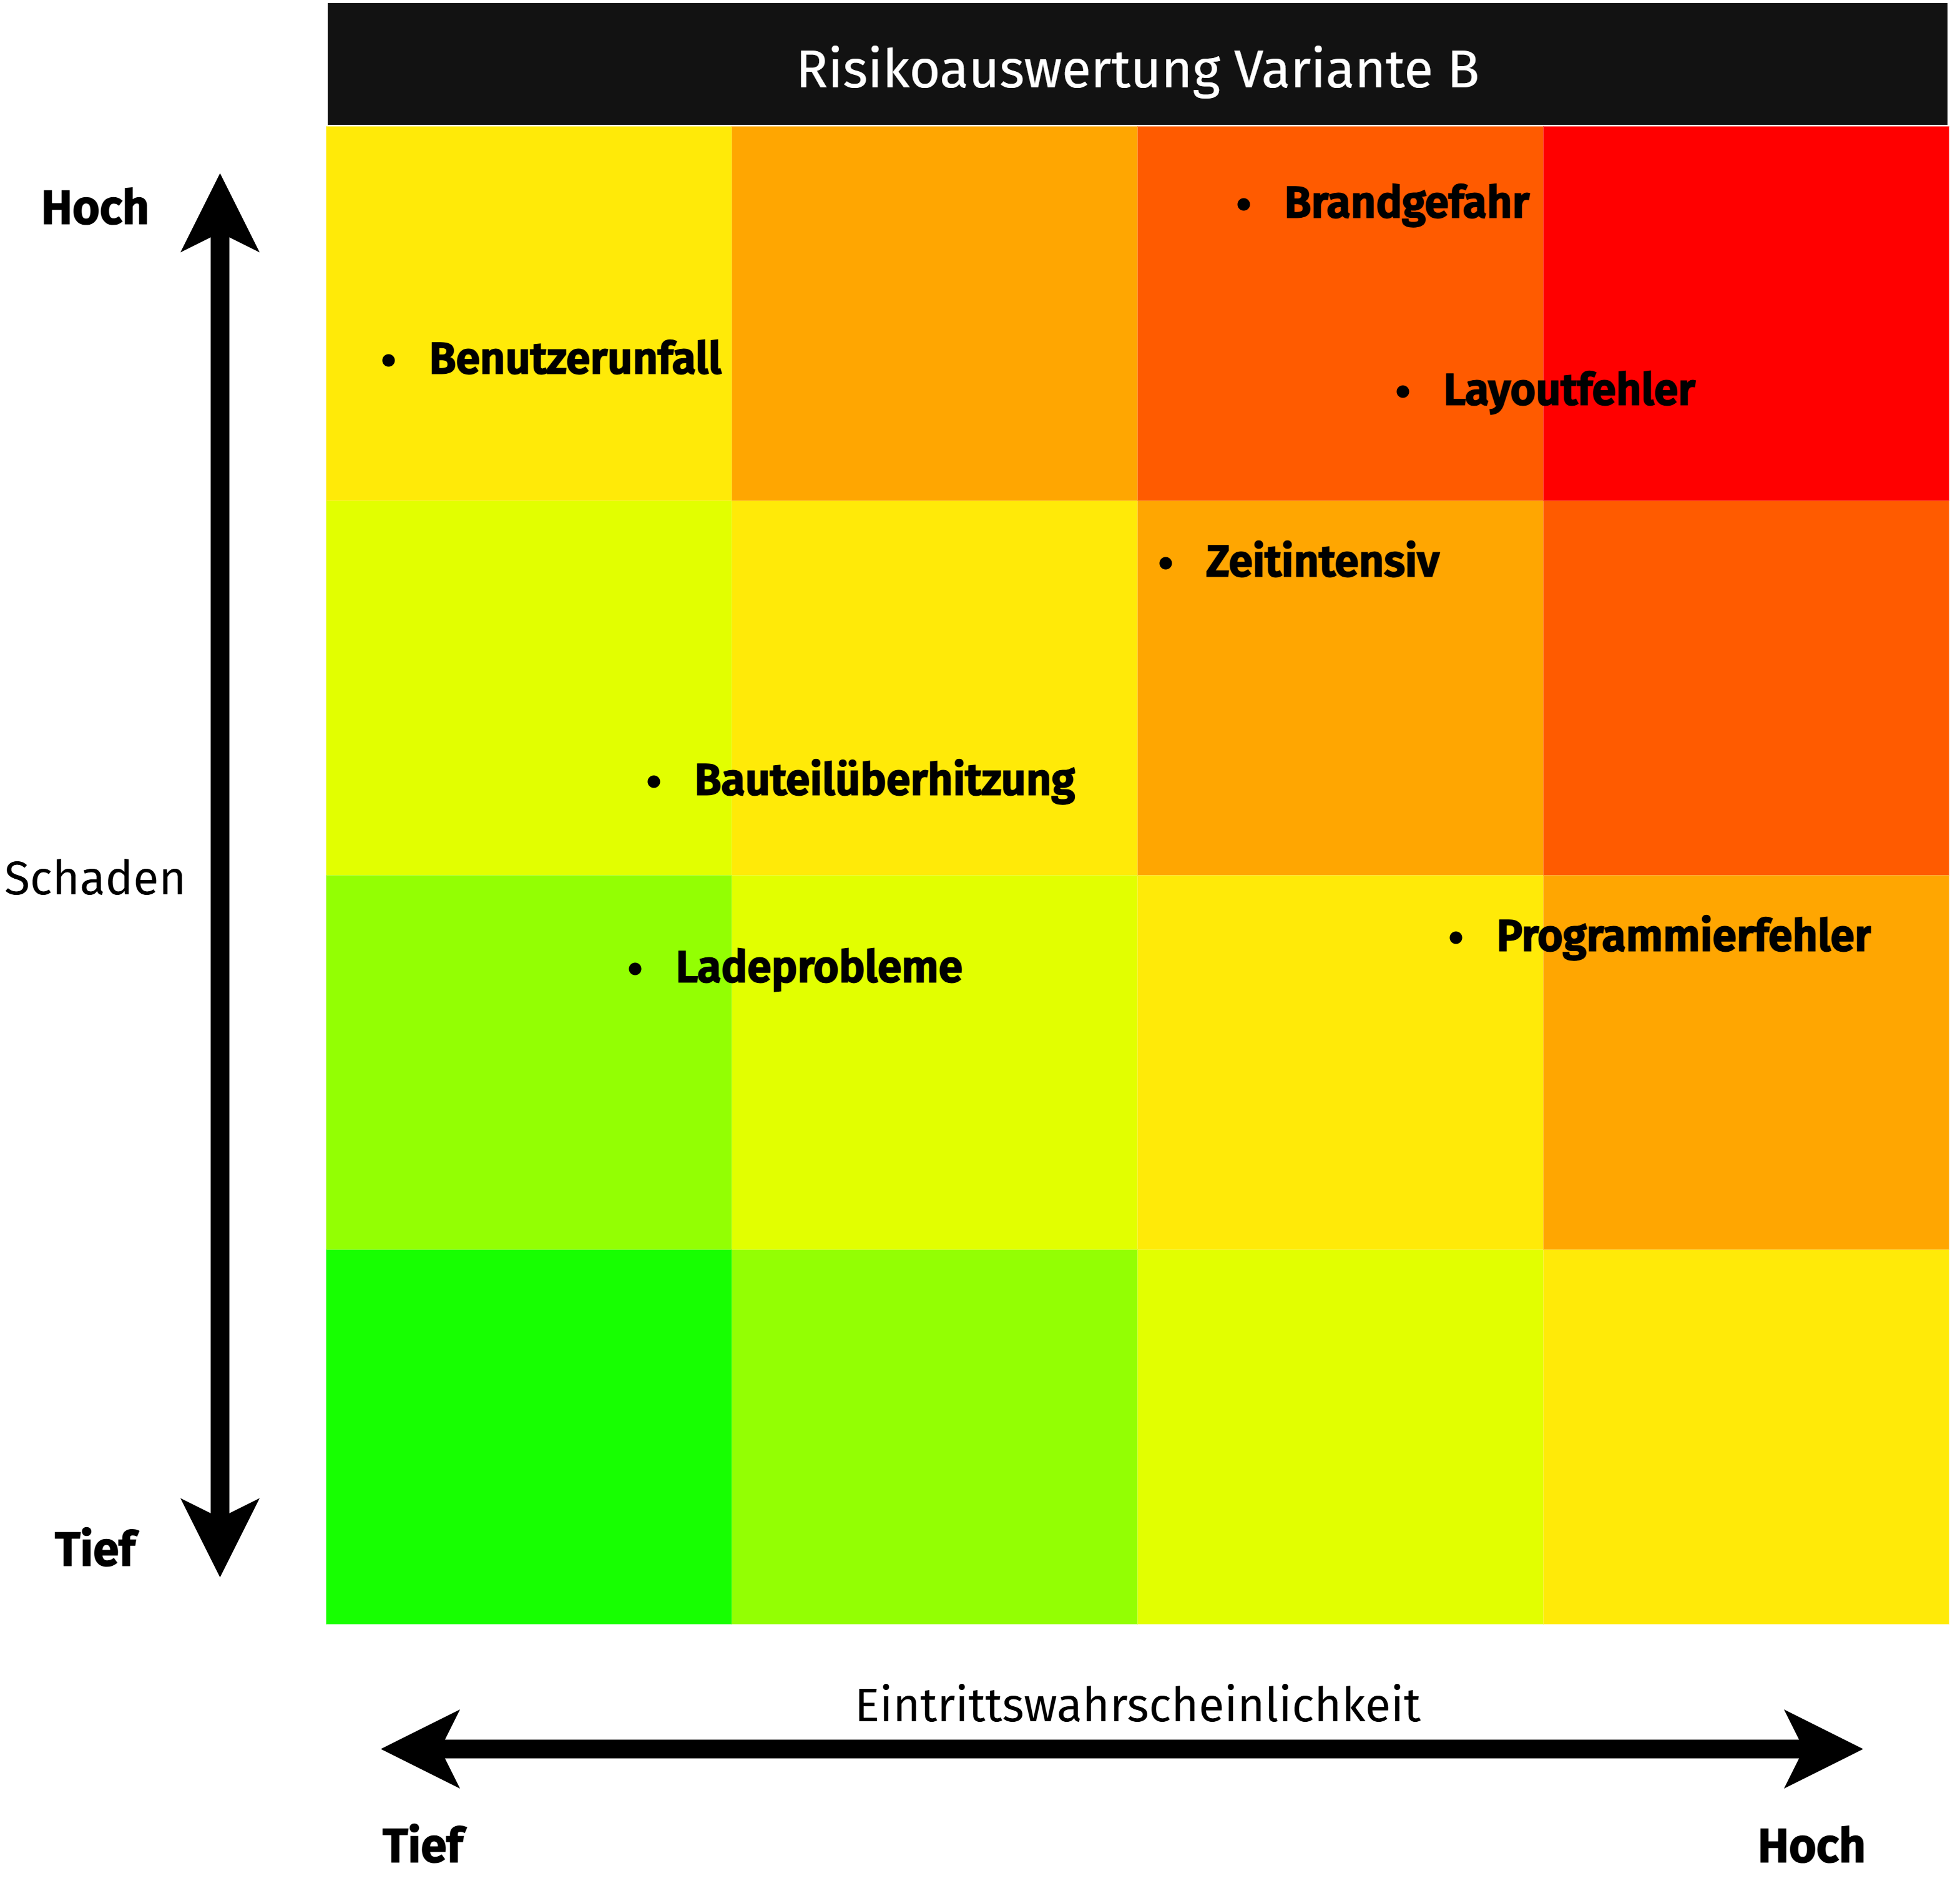
\includegraphics[width=\textwidth*4/5]{pictures/risks-Variante B_ Portabel und Drahtlos.drawio.png}
	\caption{Risikoanalyse der Variante B}
\end{figure}
\newpage
\subsubsection{Variante C: High-End Audiophil}
Maximale Kontrolle steht bei dieser Variante im Zentrum. Nur bewährte und zuverlässige Komponenten sollen verwendet werden. Einkaufsteile sind nach Verzerrungsfreiheit und rauscharmen Signalpfaden auszuwählen. Preispunkt ist sekundär.
\begin{figure}[H]
	\centering
	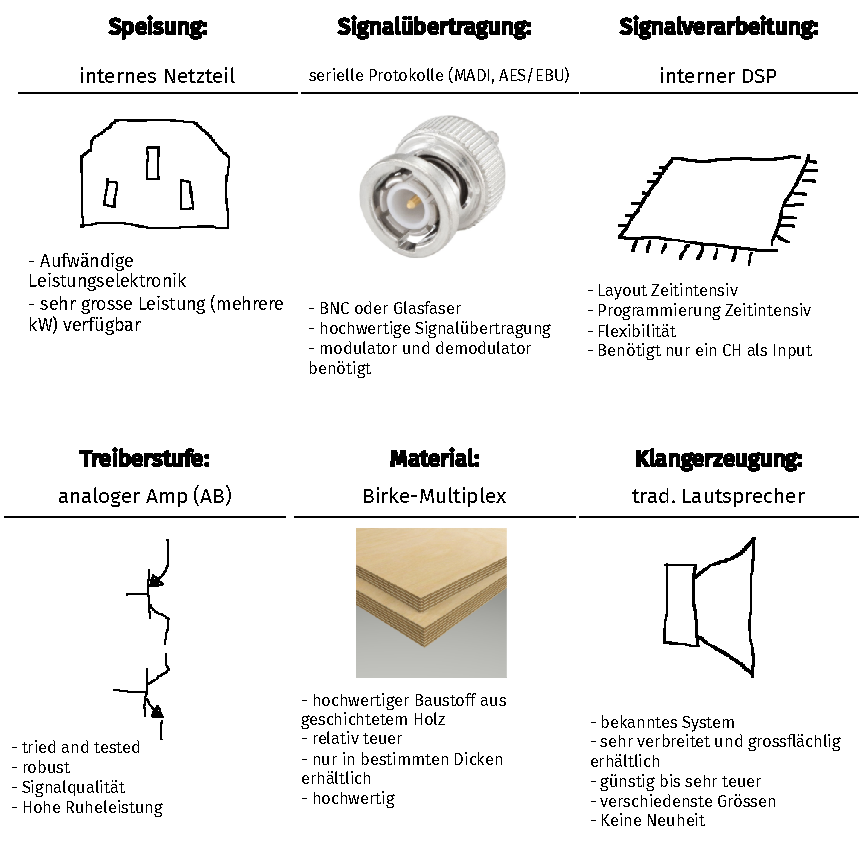
\includegraphics{pictures/VarianteC_HighEndAudiophil.pdf}
	\caption{Variante C}
\end{figure}
\paragraph{Vorteile} Die Audioqualität als oberste Priorität begünstigt ein beeindruckendes Hörerlebnis. Zudem ist die Auswahl an bewährten Methoden und robusten Materialien ein Garant für eine lange Lebensdauer.
\paragraph{Nachteile} Als erstes ist hier sicher auch die Komplexität zu nennen, da sehr spezifische Bauteile ausgewählt werden müssen, die unter Umständen nicht weit verbreitet sind. Zum anderen wird hier auch das Budget sehr strapaziert, wohl über die Belastungsgrenzen hinaus.
\newpage
\paragraph{Risikoanalyse}
Die grosse Anzahl verschiedener eigens entworfenen Komponenten führt nebst der Gefahr eines \textit{Scope Creeps} auch eventuell zu Ungenauigkeiten oder unvorhergesehenen negativen Effekten. Zudem kommt zur Leistungselektronik der Endstufe auch die Leistungselektronik des Netzteils hinzu. Auch der Lautsprecher an sich kann überhitzen und zu Brandursachen führen.
\begin{figure}[H]
	\vspace{1cm}
	\centering
	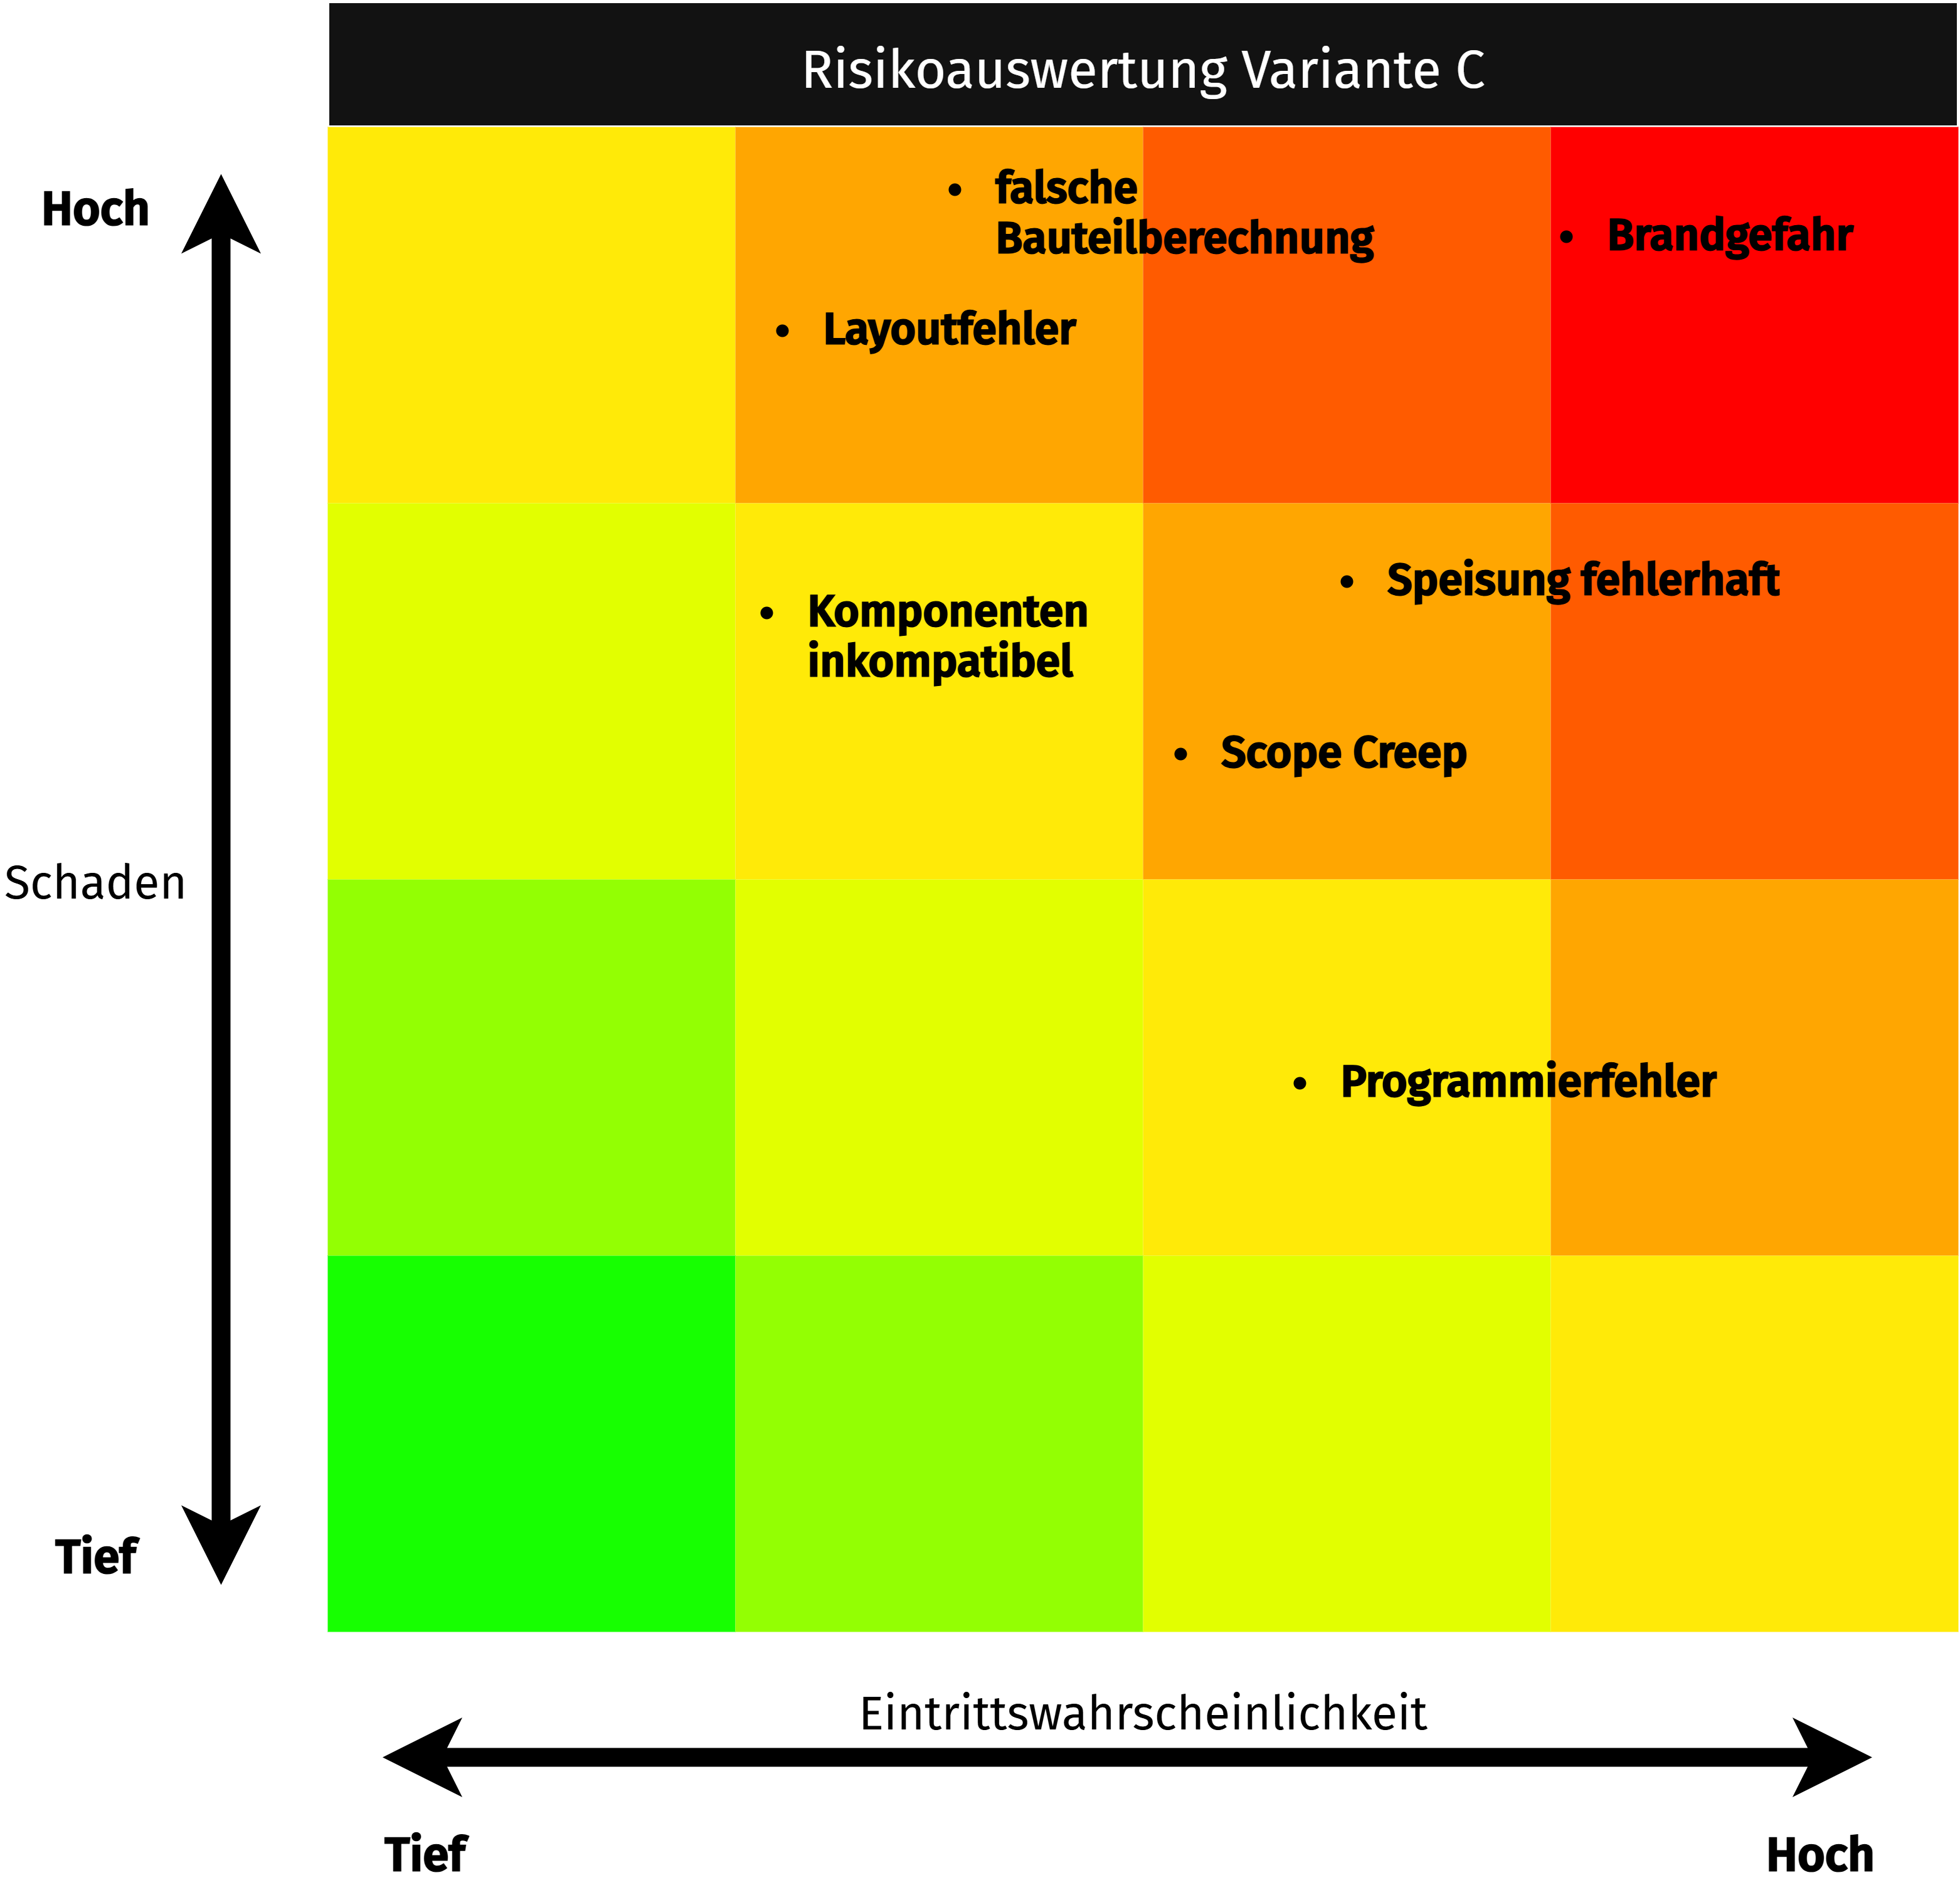
\includegraphics[width=\textwidth*4/5]{pictures/risks-Variante C.png}
	\caption{Risikoanalyse der Variante C}
\end{figure}
\newpage
\subsubsection{Variante D: Einfache Anwendung, Plug'n'Play}
Möglichst einfache Anwendung ist zentral für ein überzeugendes Benutzererlebnis. Daher wurde diese Variante mit diesem Fokus generiert. Zudem ist ein Nebenfokus hier die günstige Herstellung des Systems.
\begin{figure}[H]
	\centering
	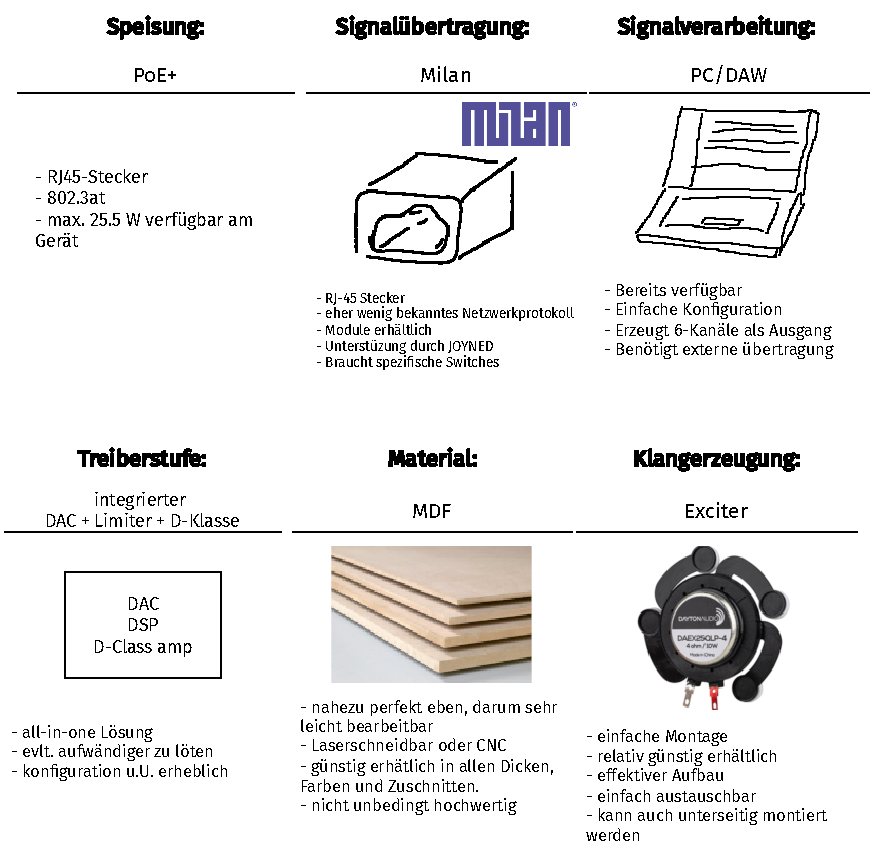
\includegraphics{pictures/VarianteD_EinfachPlugnPlay.pdf}
	\caption{Variante D}
\end{figure}
\paragraph{Vorteile} Da Datensignale und Speisung auf einem RJ45-Stecker geliefert werden, muss nur diese eine Verbindung hergestellt werden. Zudem ist mit dem MILAN-Protokoll eine automatische Bandbreitenreservation und somit keine Benutzerkonfiguration notwendig. Da DAC und Treiberstufe in einem Chip integriert ist, bleibt die Programmierung begrenzt. 
\paragraph{Nachteile} Da das Signal direkt vom PC generiert wird, muss dieses zuerst in das MILAN-Protokoll verpackt werden. Zudem muss ein AVB-fähiger Switch verwendet werden.
\newpage
\paragraph{Risikoanalyse}
Die Brandgefahr bleibt nach wie vor ein Hauptfaktor in der Risikoauswertung, bedingt durch die Verbindung von Holzfasern und Leistungsendstufen. Der noch nicht weitum verbreitete MILAN-Standard könnte hier auch zu Inkompatibilitäten, oder zumindest zu einem komplexen Setup führen. Auch könnte die Implementierung eines neuen Standards schnell \textit{Scope Creep} führen, da keine fix fertigen Lösungen bereitstehen.
\begin{figure}[H]
	\vspace{1cm}
	\centering
	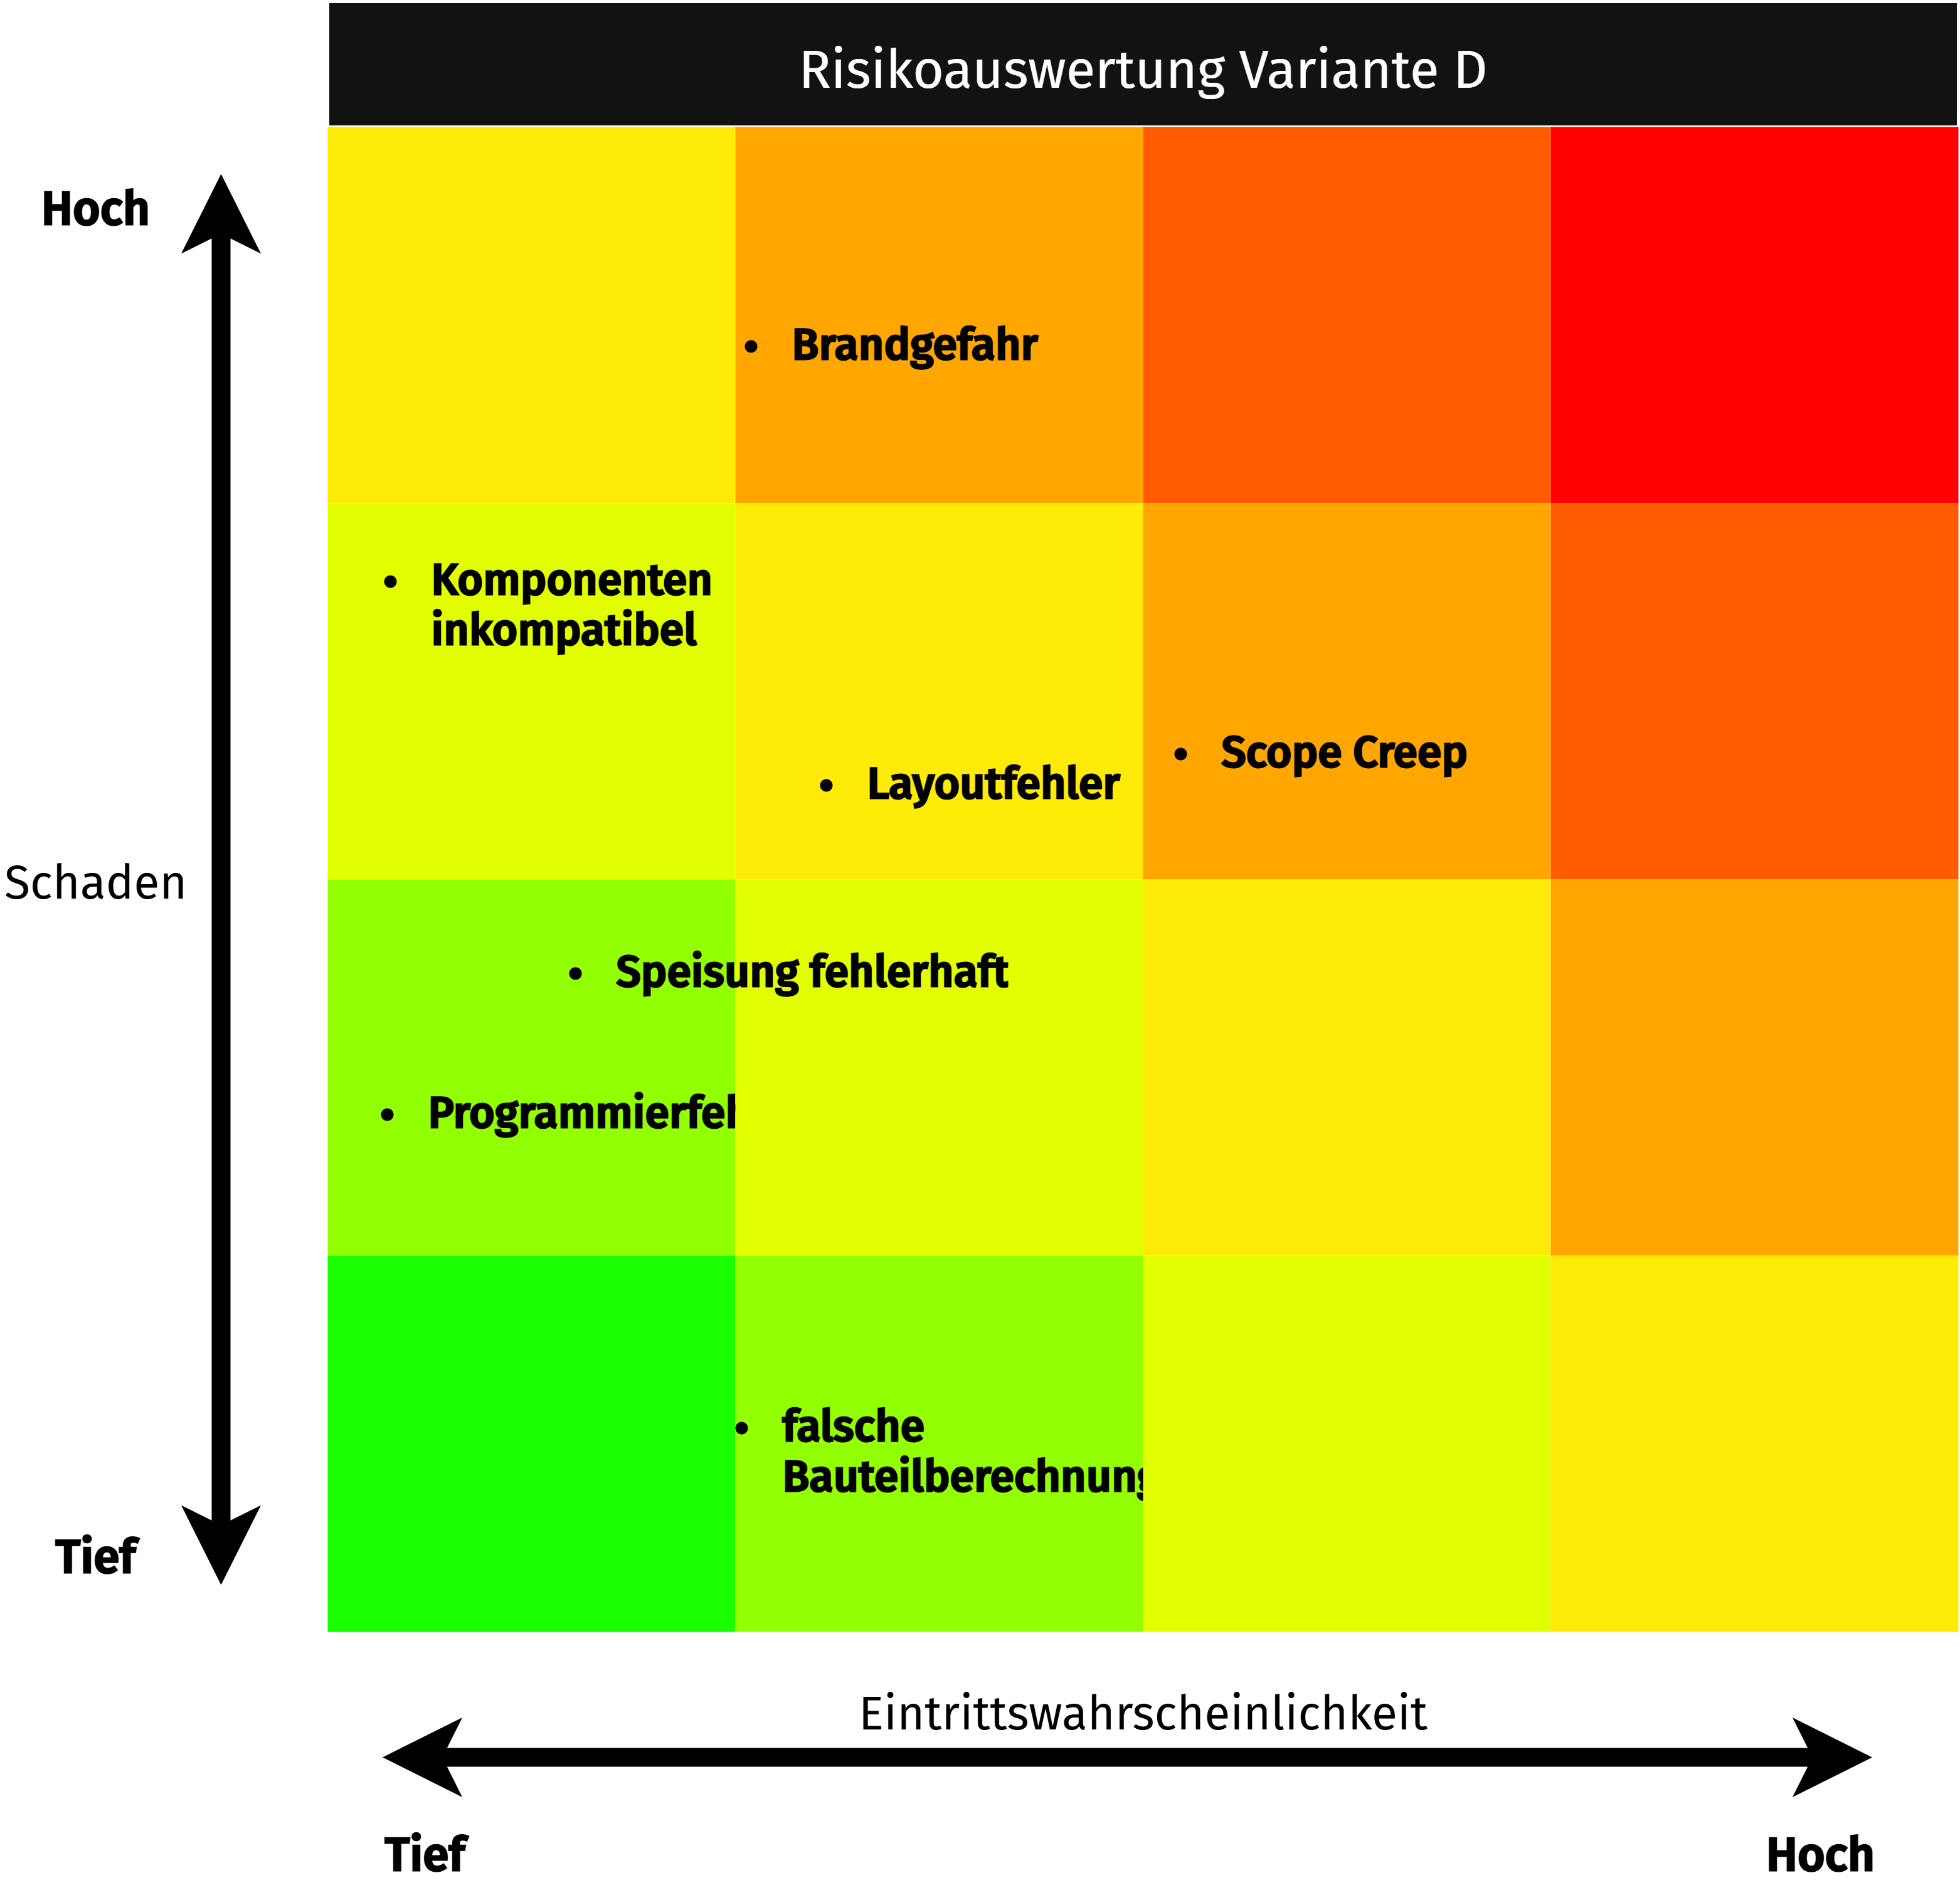
\includegraphics[width=\textwidth*4/5]{pictures/risks-Variante D.png}
	\caption{Risikoanalyse der Variante D}
\end{figure}
\newpage
\subsubsection{Variante E: Neu ist besser}
Innovation und moderne Technologie ist das Hauptmerkmal dieser Variante. Es sollen möglichst die neusten Methoden und Komponenten verwendet werden. Etablierte Verfahren sind bereits vollumfänglich im Markt vorhanden und daher uninteressant. Daher werden alles entweder neue Technologien oder bislang nicht verwendete Ideen verwendet.
\begin{figure}[H]
	\centering
	\includegraphics{pictures/VarianteE_Neuistbesser.pdf}
	\caption{Variante E}
\end{figure}
\paragraph{Vorteile} Durch die Neuheit und Innovation entsteht Freiheit: Es gibt in dem Sinne keine etablierte Verfahren oder Protokolle. Daher eröffnet sich ein Spielraum für Eigeninitiative.
\paragraph{Nachteile} Durch die undefinierten Variablen muss sehr viel Arbeit in deren Ausarbeitung investiert werden. So muss die gesamte Signalverarbeitung und die Kommunikation mit dem DAC definiert werden. Zudem entstehen unter Umständen weitere Kosten durch wenig verfügbare Bauteile.
\newpage
\paragraph{Risikoanalyse}
Nebst hohen Herstellungskosten kann hier eine stromdurchflossene Saite erhitzen und zu Verbrennungen führen. Des weiteren kann die Impedanz der Saite schlicht zu tief sein für die Endstufe, wodurch die Schwingung wenn überhaupt nur kaum wahrnehmbar also extrem leise erzeugt werden kann. Zudem entsteht durch den internen DSP auch hier die Gefahr des \textit{Scope Creep}, da die Signalverarbeitung potentiell recht umfangreich werden kann.
\begin{figure}[H]
	\vspace{1cm}
	\centering
	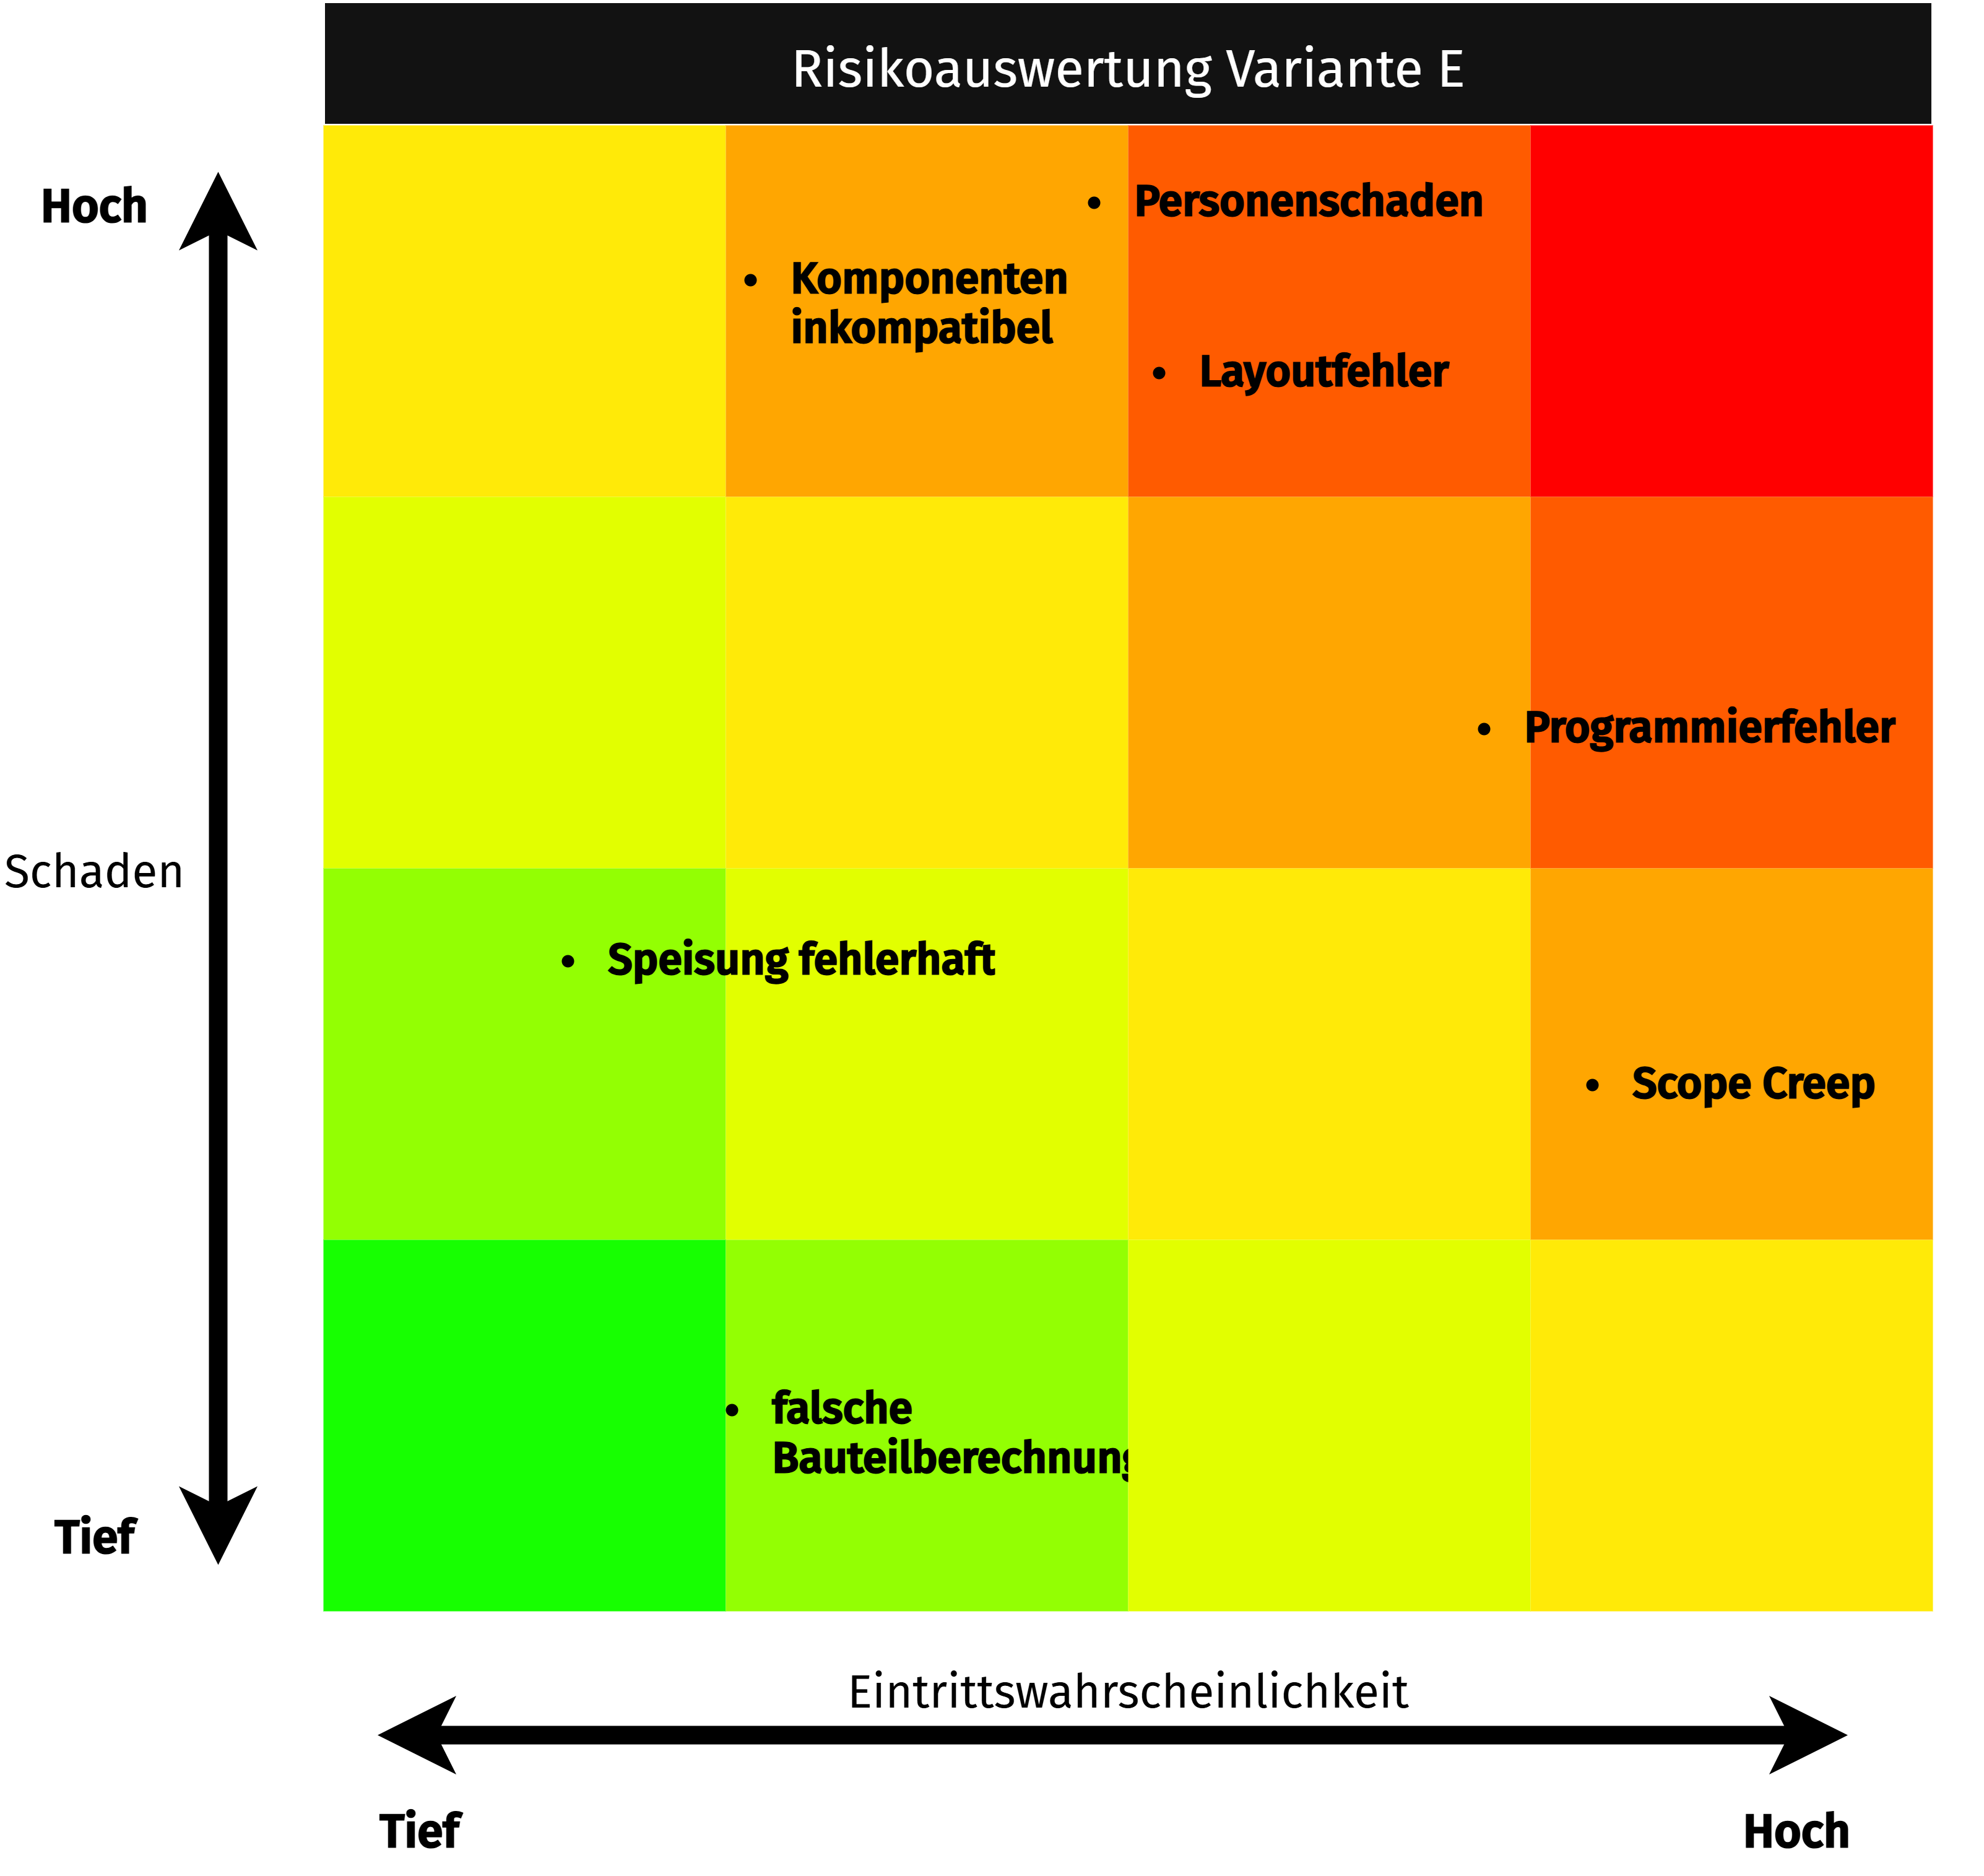
\includegraphics[width=\textwidth*4/5]{pictures/risks-Variante E.png}
	\caption{Risikoanalyse der Variante E}
\end{figure}
\newpage
\section{Variantenauswertung}
\subsubsection{Nutzwertanalyse}Zur Auswertung wurde eine Nutzwertanalyse durchgeführt, bei der die Primärkriterien auf Erfüllung oder Nichterfüllung hin geprüft wurden. Idealerweisen sollten dabei alle Primärziele erfüllt werden. Alle anderen Ziele wurden gemäss Tabelle \ref{tab:zielgewichtung} neu gewichtet und deren Erfüllung mit einer Note von 1 bis 10 und bei Nichterfüllung 0 bewertet. Die Multiplikation der Gewichtuung mit der Note ergibt ein Zwischenresultat für ein Ziel. Die Summe der Zwischenresultate ergibt die Gesamtpunktzahl nach Sekundärzielen. Diese Analyse ist in Abbildung \ref{pic:nutzwertanalyse} dargestellt. Mit diesen Kriterien erfüllt nur \textbf{Variante D} die Muss-Ziele.
\subsubsection{Kosten-Nutzen Analyse}
In Bezug zu den verwendeten Komponenten und Materialien kann eine Schätzung für die Kosten jeder Variante abgegeben werden:
\begin{itemize}
	\item \textbf{Variante A: Alles Analog}: Hoch, vor allem durch den Zeitaufwand
	\item \textbf{Variante B: Drahtlos \& Portabel}: Mittel, jedoch PMMA als Preistreiber
	\item \textbf{Variante C: High-End Audiophil}: Sehr hoch, durch Spezial- und High-End Komponenten
	\item \textbf{Variante D: Einfache Anwendung, Plug’n’Play}: Tief-Mittel
	\item \textbf{Variante E: Neu ist besser}: Mittel, jedoch PMMA und Zeitaufwand
\end{itemize}
Diese Erkenntnis kann auf die in der Nutzwertanalyse erreichte Punktzahl abgebildet werden. Abbildung \ref{pic:kostennutzen} zeigt dieses Verhältnis grafisch auf. Dabei sind Lösung mit Tendenz in Richtung untere rechte Ecke (\textit{hoher Nutzen, tiefe Kosten}) zu bevorzugen. Dagegen sind Lösungen mit Tendenz Richtung oberen linke Ecke mit hohen Kosten, aber wenig Nutzen verbunden.
\begin{figure}[H]
	\centering
	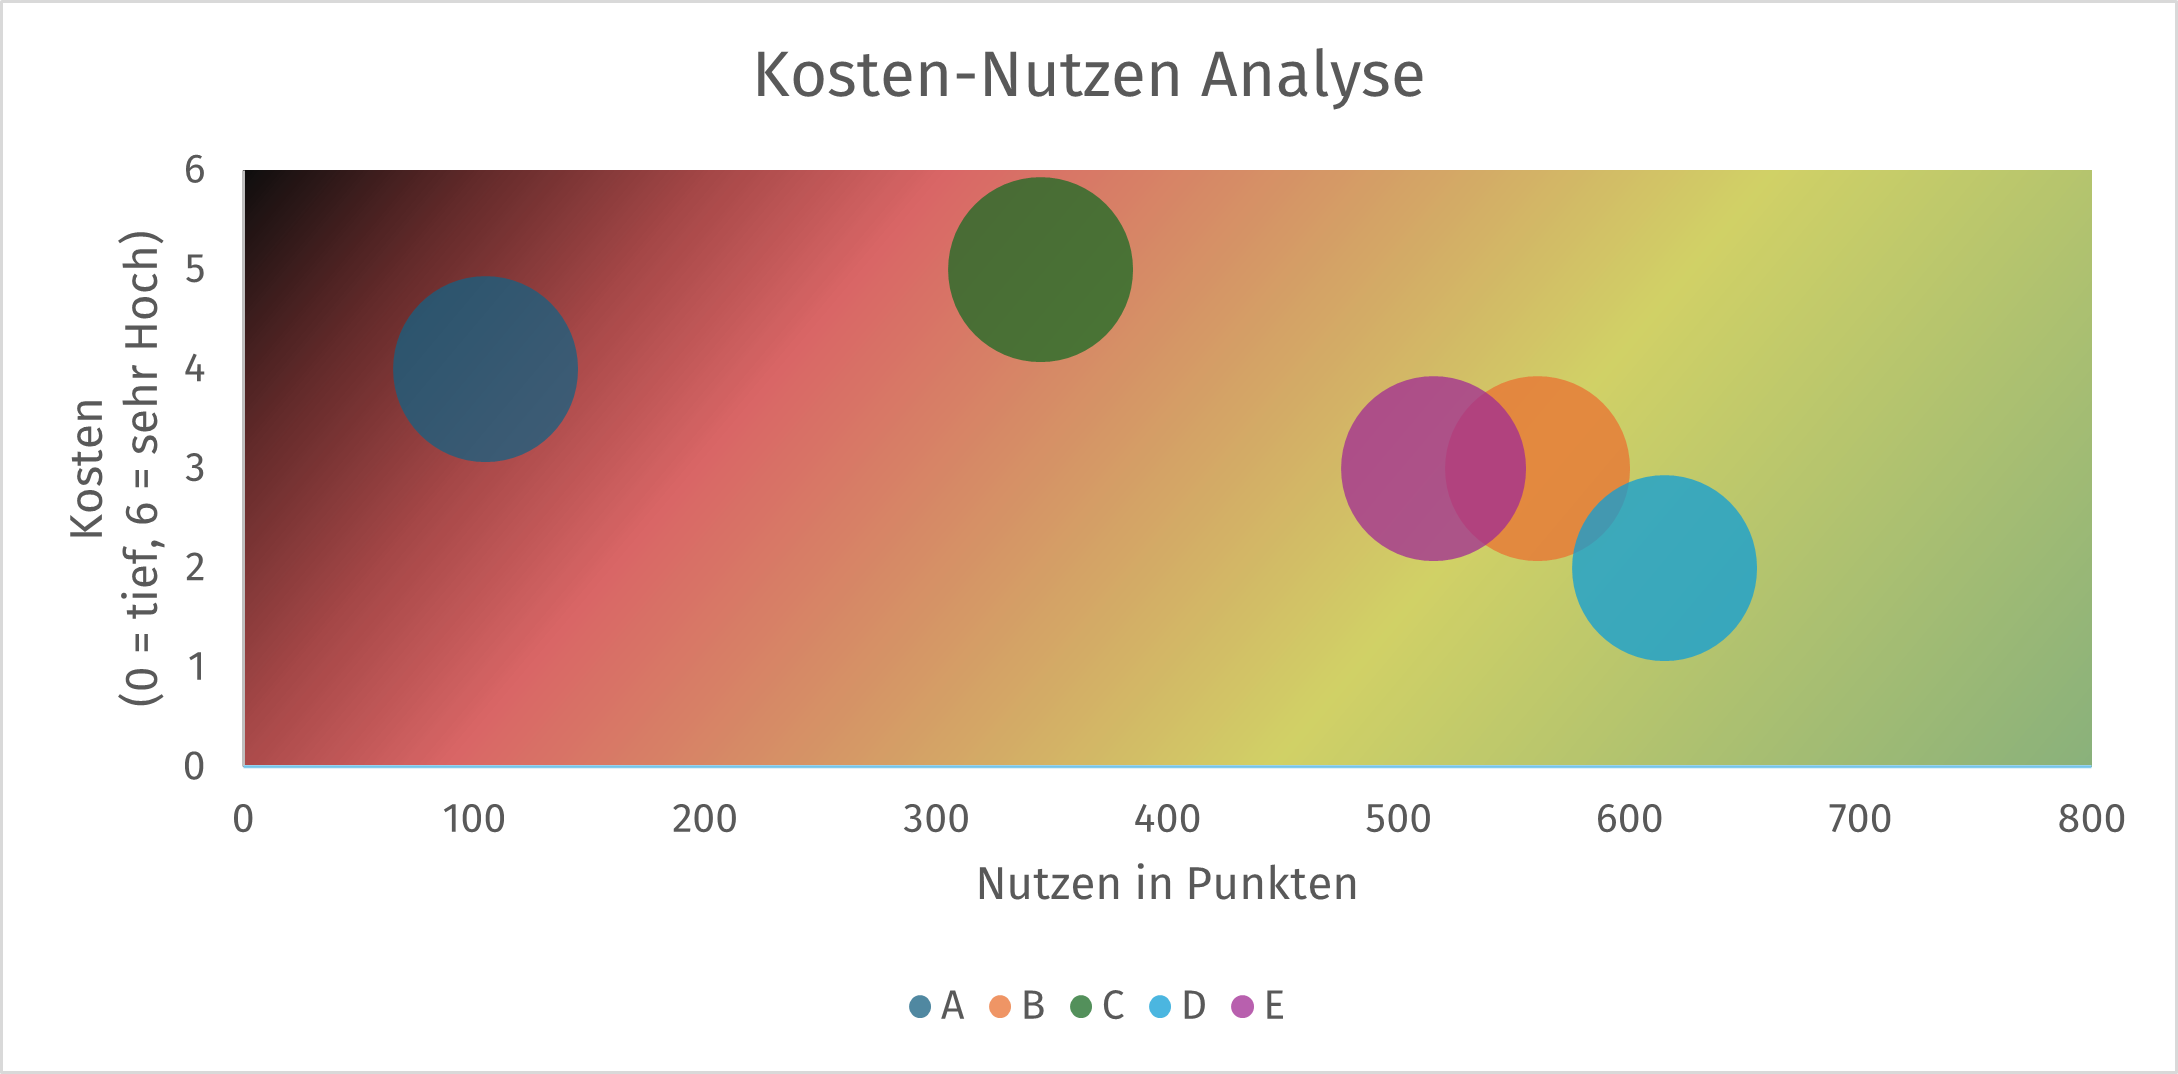
\includegraphics[width=\textwidth - 2cm]{pictures/Kostennutzenanalyse.png}
	\caption{Kosten-Nutzen Analyse}
	\label{pic:kostennutzen}
\end{figure}
\newpage
\begin{figure}[H]
	\centering
	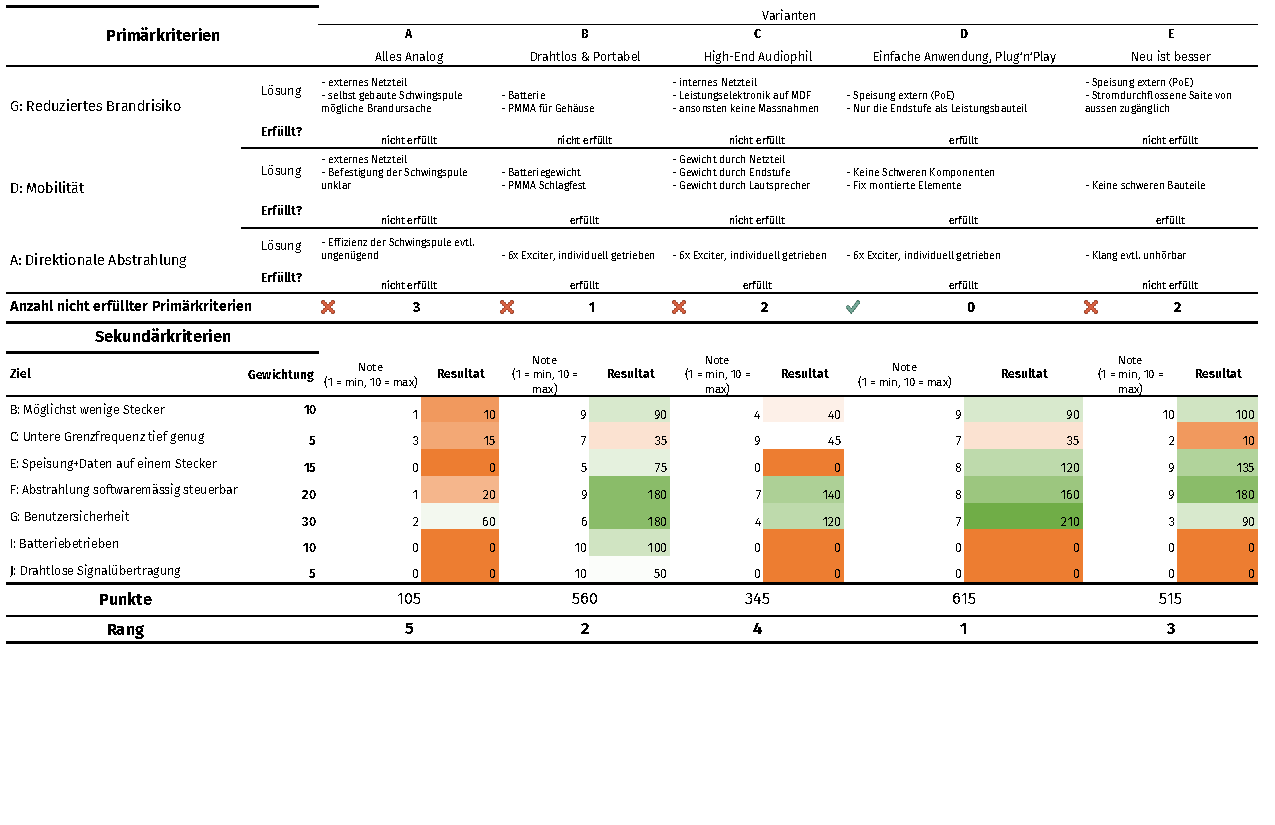
\includegraphics[trim={0 3cm 0 0},clip,width=\textheight - 1cm, angle=90]{pictures/Nutzwertanalyse.pdf}
	\caption{Nutzwertanalyse}
	\label{pic:nutzwertanalyse}
\end{figure}
\newpage
\section{Variantenauswahl}
Die Variantenanalysen zeigt klar, dass \textbf{Variante D: Einfache Anwendung} aus Risikogründen, Nutzwertanalyse und der Kosten-Nutzen die vielversprechendste Variante ist. Die Kombination aus fixfertigen Modulen, wenigen Neuentwicklungen und wenigen Komponenten führt in vielen Belangen zu vorteilhaften Eigenschaften. Ein weiterer Vorteil ist, dass durch den Einsatz von Excitern sich die Konstruktion erheblich vereinfacht, da keine Saite gespannt oder fixiert werden muss und keine sich bewegende Teile von aussen zugänglich sind.
\paragraph{Anpassungen}Nichtsdestotrotz kann diese Variante noch weiter optimiert und kombiniert werden. So können zum Beispiel mehrere Materialien für das Gehäuse verwendet werden. Daher wurde diese Variante auf die Primärziele hin noch weiter angepasst. Nachfolgend sind daher die Primärziele mit den entsprechenden Massnahmen aufgelistet:\\
\begin{figure}[H]
	\centering
	\setstretch{1.5}
	\begin{tabularx}{\textwidth*4/5}{lX}
		{\large \textbf{Ziel}} & {\large Massnahme}\\
		\midrule\vspace{-6mm}\\
		\textbf{G: Reduziertes Brandrisiko}&Montage der stromführenden Bauteile auf PMMA\\
		\vspace{2mm}\textbf{D.2: Mobilität}&Einsatz eines externen USB-MILAN Dongles für die Verbindung zwischen PC und Gerät. Somit ist kein Switch vonnöten.\\
		\vspace{2mm}\textbf{A: Direktionale Abstrahlung}&Externes Netzteil für grösseres Leistungsbudget\\
		\bottomrule
	\end{tabularx}
	\caption{Weitere Massnahmen}
\end{figure}


\section{Terminplanung}
\begin{table}[!ht]
	\centering
	\caption{Terminplanung in tabellarischer Form}
	\setstretch{1.5}
	\begin{tabularx}{388pt}{|l|l|l|l|}
		\textbf{Arbeitspaket} & \textbf{URL} & \textbf{Startdatum} & \textbf{Enddatum} \\\hline
		\textbf{Terminplanung} & \href{https://github.com/Violabitch5/Nathophone\_doc/issues/1}{Link} & Sep 4, 2025 & Sep 5, 2025 \\ 
		\textbf{IST-Zustandsanalyse} & \href{https://github.com/Violabitch5/Nathophone\_doc/issues/4}{Link} & Sep 6, 2025 & Sep 7, 2025 \\ 
		\textbf{Zieldefinition} & \href{https://github.com/Violabitch5/Nathophone\_doc/issues/3}{Link} & Sep 8, 2025 & Sep 9, 2025 \\ 
		\textbf{Zielgewichtung} & \href{https://github.com/Violabitch5/Nathophone\_doc/issues/5}{Link} & Sep 10, 2025 & Sep 11, 2025 \\ 
		\textbf{Varianten- \& Risikoanalyse} & \href{https://github.com/Violabitch5/Nathophone\_doc/issues/6}{Link} & Sep 12, 2025 & Sep 16, 2025 \\ 
		\textbf{Variantenauswahl} & \href{https://github.com/Violabitch5/Nathophone\_doc/issues/7}{Link} & Sep 17, 2025 & Sep 17, 2025 \\ 
		\hdashline
		\textbf{Kennzahlberechnung / Limits} & \href{https://github.com/Violabitch5/Nathophone\_elec/issues/1}{Link} & Sep 18, 2025 & Sep 21, 2025 \\ 
		\textbf{Bauteileevaluation} & \href{https://github.com/Violabitch5/Nathophone\_elec/issues/2}{Link} & Sep 22, 2025 & Sep 30, 2025 \\ 
		\textbf{Bauteilauswahl} & \href{https://github.com/Violabitch5/Nathophone\_elec/issues/3}{Link} & Oct 1, 2025 & Oct 4, 2025 \\ 
		\textbf{Print Schema draft} & \href{https://github.com/Violabitch5/Nathophone\_elec/issues/4}{Link} & Oct 5, 2025 & Oct 11, 2025 \\ 
		\textbf{Print Schema v1} & \href{https://github.com/Violabitch5/Nathophone\_elec/issues/5}{Link} & Oct 12, 2025 & Oct 18, 2025 \\ 
		\textbf{Print Layout v1} & \href{https://github.com/Violabitch5/Nathophone\_elec/issues/6}{Link} & Oct 19, 2025 & Oct 26, 2025 \\ 
		\textbf{Peer-review Schema und Layout} & \href{https://github.com/Violabitch5/Nathophone\_elec/issues/7}{Link} & Oct 27, 2025 & Oct 31, 2025 \\ 
		\textbf{Print Schema Final} & \href{https://github.com/Violabitch5/Nathophone\_elec/issues/8}{Link} & Nov 1, 2025 & Nov 3, 2025 \\ 
		\textbf{Print Layout final} & \href{https://github.com/Violabitch5/Nathophone\_elec/issues/9}{Link} & Nov 3, 2025 & Nov 6, 2025 \\ 
		\textbf{Gerber-Daten generieren und Printbestellung} & \href{https://github.com/Violabitch5/Nathophone\_elec/issues/10}{Link} & Nov 7, 2025 & Nov 7, 2025 \\ 
		\textbf{Konstruktion des Korpus fertigstellen} & \href{https://github.com/Violabitch5/Nathophone\_mech/issues/1}{Link} & Nov 8, 2025 & Nov 10, 2025 \\ 
		\textbf{Herstellung Korpus-Teile} & \href{https://github.com/Violabitch5/Nathophone\_mech/issues/2}{Link} & Nov 11, 2025 & Nov 15, 2025 \\ 
		\textbf{Zusammenbau Korpus} & \href{https://github.com/Violabitch5/Nathophone\_mech/issues/3}{Link} & Nov 16, 2025 & Nov 22, 2025 \\ 
		\textbf{Bestückung + Lötarbeit Print} & \href{https://github.com/Violabitch5/Nathophone\_elec/issues/11}{Link} & Nov 23, 2025 & Nov 30, 2025 \\ 
		\textbf{Funktionstest Print} & \href{https://github.com/Violabitch5/Nathophone\_elec/issues/12}{Link} & Dec 1, 2025 & Dec 4, 2025 \\ 
		\textbf{Zusammenbau Komplettsystem} & \href{https://github.com/Violabitch5/Nathophone\_mech/issues/4}{Link} & Dec 4, 2025 & Dec 18, 2025 \\ 
		\textbf{Funktionstests Komplettsystem} & \href{https://github.com/Violabitch5/Nathophone\_elec/issues/13}{Link} & Dec 18, 2025 & Dec 25, 2025 \\ 
		\textbf{Schlussmessung \& Auswertungen} & \href{https://github.com/Violabitch5/Nathophone\_elec/issues/14}{Link} & Dec 25, 2025 & Dec 31, 2025 \\ 
		\hdashline
		\textbf{Audruck (Plakat und Arbeit)} & \href{https://github.com/Violabitch5/Nathophone\_doc/issues/8}{Link} & Jan 1, 2026 & Jan 6, 2026 \\ 
		\textbf{Abgabe Diplomarbeit} & \href{https://github.com/Violabitch5/Nathophone\_doc/issues/2}{Link} & Jan 7, 2026 & Jan 7, 2026
	\end{tabularx}
	\label{terminplan}
\end{table}
\vspace{-4mm}
%--- Theory -------------------------------------

%--- Umsetzung -----------------------------------------
\section{Umsetzung}
%\input{doc_implementation.tex}
\subsection{Systemaufbau}
%\input{doc_systemstructure.tex}
\section{Tests}
%\input{doc_tests.tex}
%--- Fazit --------------------------------------------
\section{Fazit}
%\input{doc_fazit.tex}
%--- Hilfsmittelverzeichnis ---------------------------
%\newpage
%\section{Hilfsmittelverzeichnis}

%--- Tabellenverzeichnis ------------------------------
\newpage
\setlength{\cftbeforelottitleskip}{0pt} % Abstand vor dem Titel des Tabellenverzeichnisses
\setlength{\cftafterlottitleskip}{15pt} % Abstand nach dem Titel des Tabellenverzeichnisses
\listoftables
\addcontentsline{toc}{section}{13 Tabellenverzeichnis}  % Fügt es zum Inhaltsverzeichnis hinzu

% --- Quellenverzeichnis ------------------------------
%\newpage
\renewcommand{\bibname}{Quellenverzeichnis}
\printbibliography[title={Quellenverzeichnis}]
\addcontentsline{toc}{section}{Quellenverzeichnis}  

\appendix

%\renewcommand{\thechapter}{\alph{chapter}}
\end{document}
% <-- end of file